\chapter{Negotiating researcher and participant relationships}
\label{NegotatingReseacherParticipantRelationships}

Before you get into the good bit, In the introduction, I will have a clear description of what chapter tackles what for the research questions and this diagram below. I will then return to the research questions in more detail in the discussion.

\begin{figure}[htp]
\centering
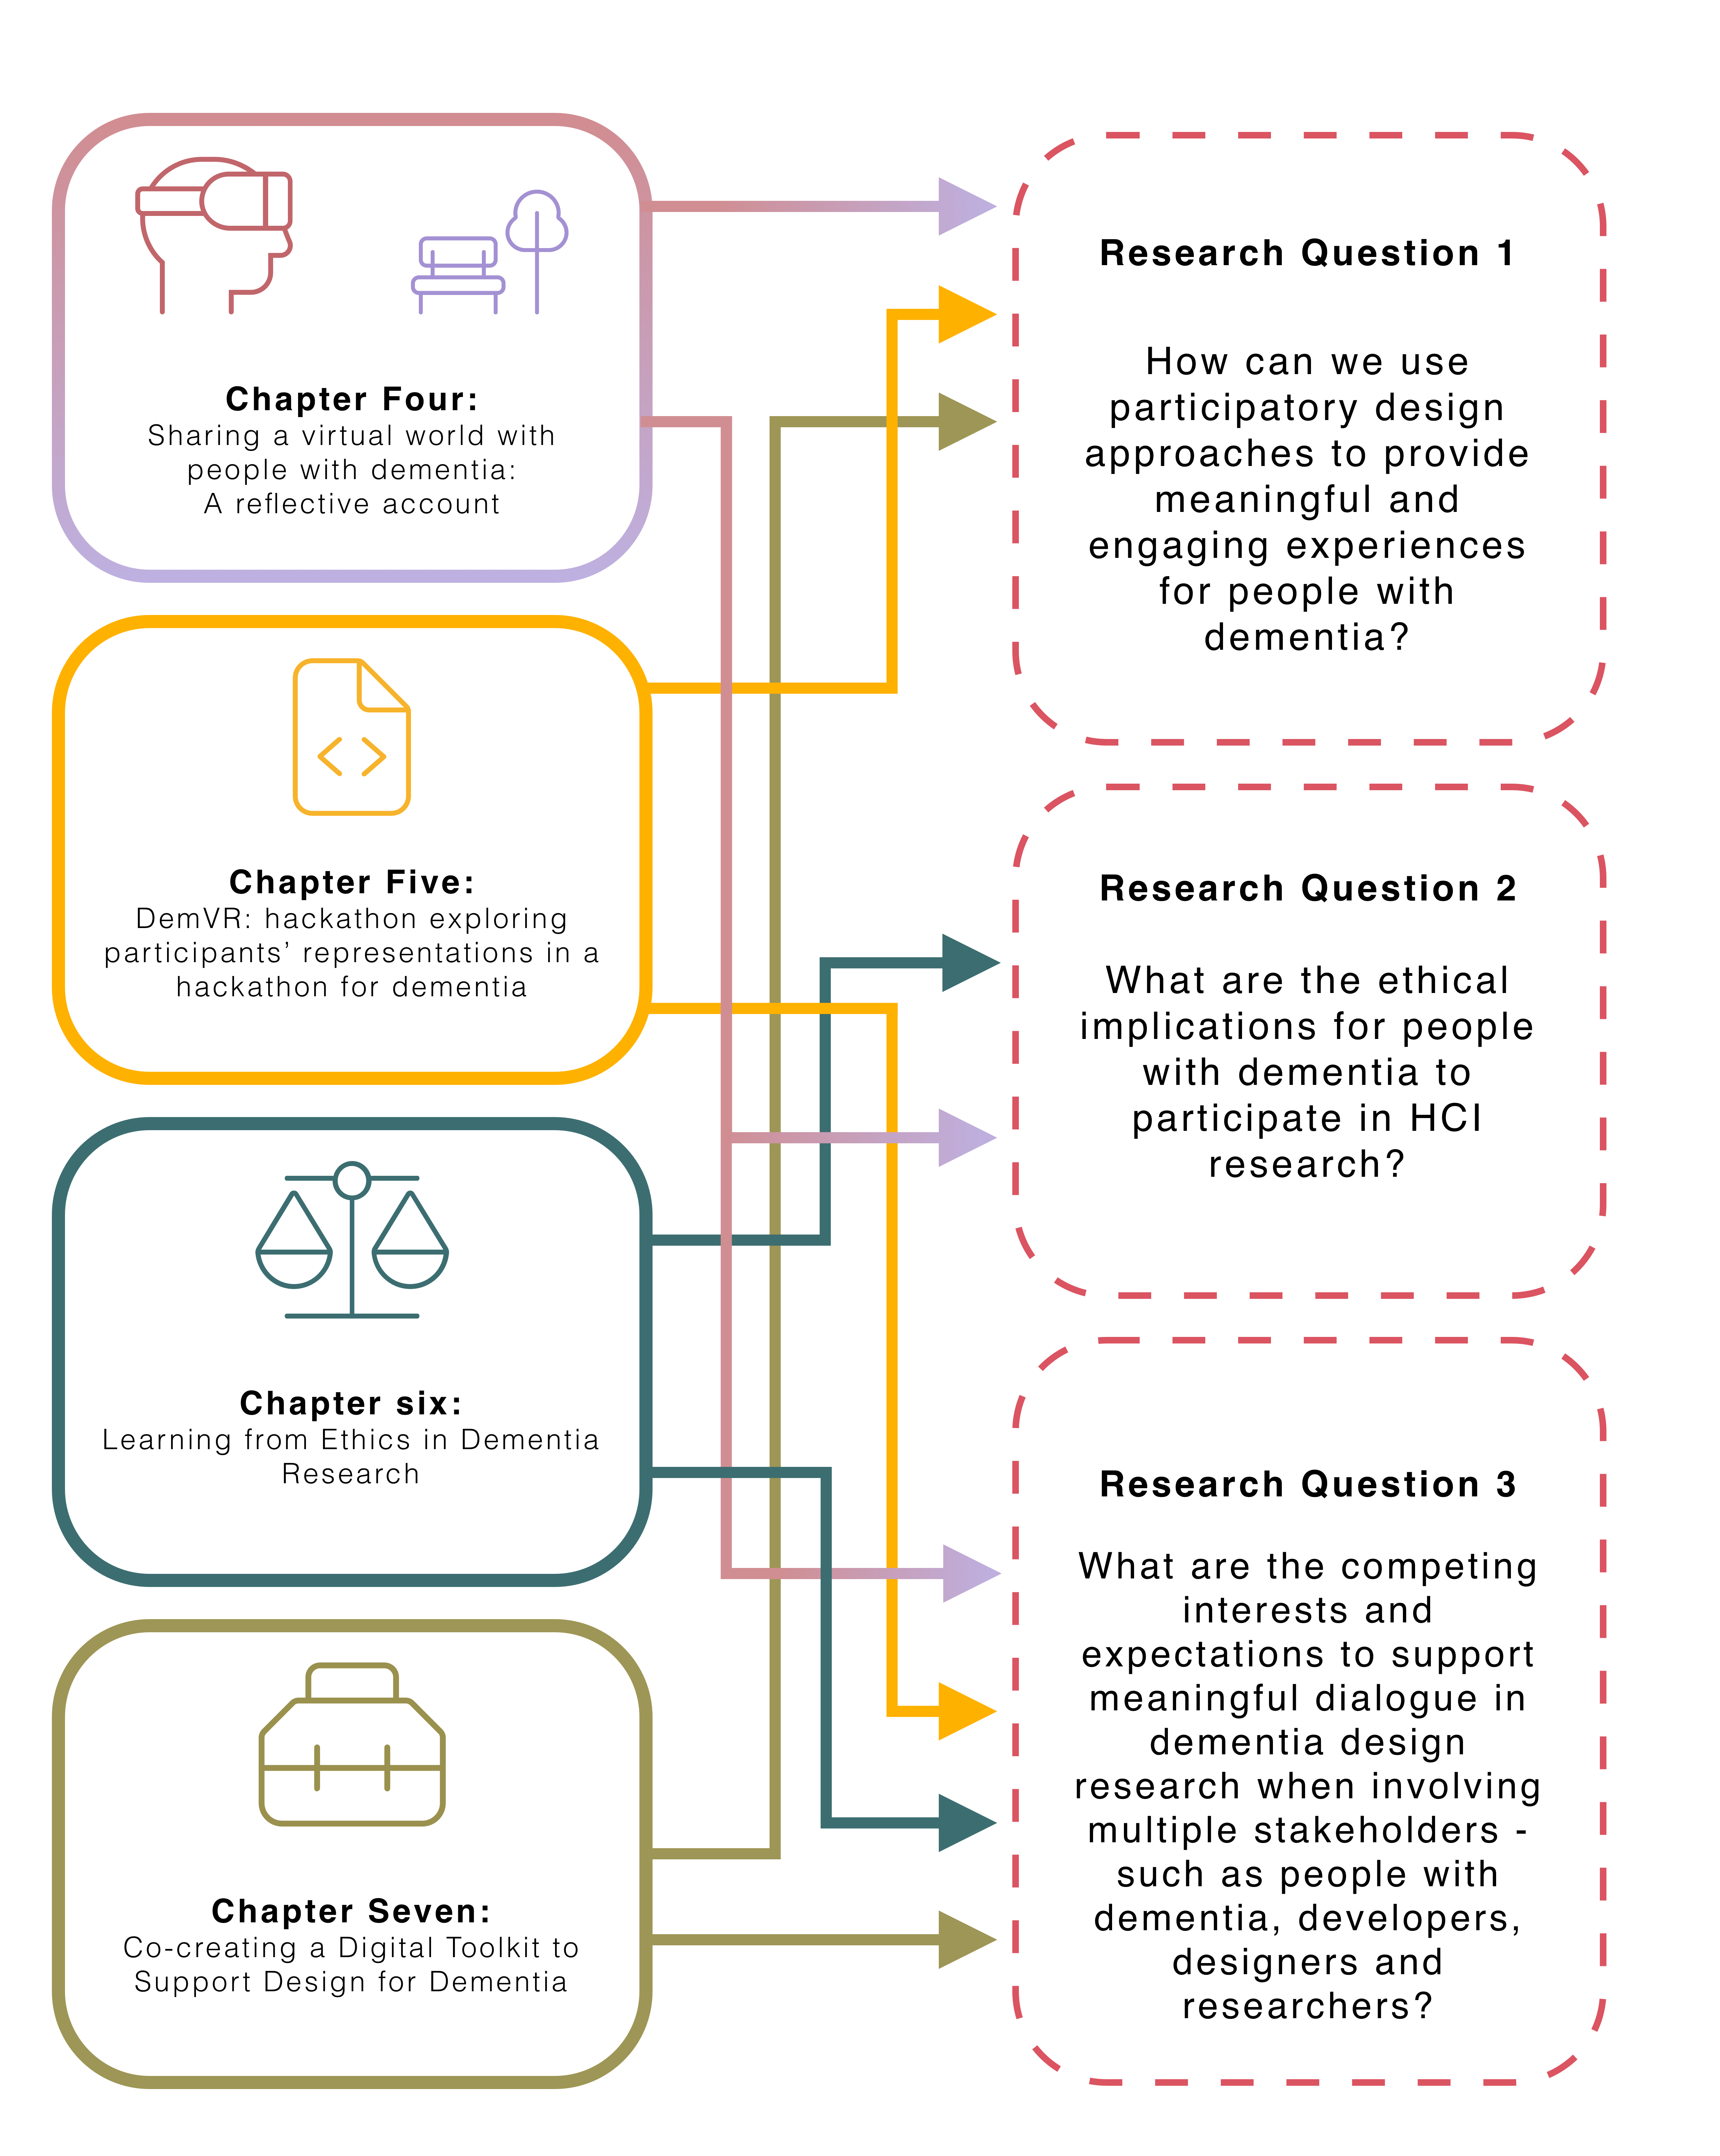
\includegraphics[width=.8\linewidth]{Images/Thesis_Narrative/RQ_and_Chapters.png}
\caption{Thesis Map showing the relationships between data chapters to research questions}
\label{fig:RQ_and_Chapters}
\end{figure}

\section{Introduction}
\label{Relationships:Introduction}
In the previous two chapters, I described the relevant literature to the context of dementia and HCI that emphasises involving people with dementia in technology design processes. Within my methodology, I highlight the ways researchers and designers have tailored participation for people with dementia - that I adopt and adapt to suit the needs of my participants within this chapter. As discussed in the two chapters, the relationship between the researcher and participant is an important one that mirrors the ethics of care in dementia research \cite{hamington_integrating_2019}. \cite{robertson2012ethics} describe the four ethical aspects of PD that influence the research partnership:
\begin{itemize}
\item Who do we engage with in a Participatory Design project?
\item How do we engage with participants?
\item How do we represent participants and their work?
\item What can we offer participants?
\end{itemize}

To explore these broader ethical questions, researchers have proposed approaches to reflect on their experiences working within these sensitive spaces to explore how design decisions play a role in the research partnerships. This chapter describes a three-year auto-ethnography that explores my path into designing in dementia and HCI research. Through two studies, I reflect on guidance into designing media and VR experiences \textit{for} and \textit{with} people with dementia. As I recall the prior three years, there is a gradual shift from VR technology being a critical part of the research, to placing importance on the broader concerns about ethics in the community of practice. For example, how does short-term memory, need for care, orientation, and a culture of ethical 'protectionism' impact the involvement of people with dementia in research. This chapter covers two- and half-year engagement with a dementia café in Newcastle known as Silverline Memories. This local registered charity prides itself on its activities, organising celebrations for members' birthdays and other special occasions. With designing for creativity becoming an essential shift in design research in dementia \citep{john_killick_claire_craig_creativity_2012,morrissey_creative_2015,wallace_design-led_2013}, the potential for VR for people living with dementia may come hand-in-hand with ways to experience and express creativity. In the first study, I explore designing tailored VR experiences, which leads to exploring how we design for media capture of meaningful experiences to support families living with dementia.

With this in mind, this chapter reveals reflective insights into how power differences shaped collaboration; the sharing of personal stories that are perhaps irrelevant to the research questions; technology appropriateness vs novelty in technology; and building of trust participants had towards myself (the researcher). Furthermore, the insights that I share in this chapter are significantly influential in the trajectory of where this thesis goes. As mentioned earlier, my work in dementia originally started with an interest in VR. However, through personal experience in conducting research, my interests lie in understanding the broader concerns of ethics in practice and how relational approaches can be structured between people with dementia and technologists who ultimately make design decisions through design and development roles.


The two studies covered in this chapter were peer-reviewed and published at the CHI Conference on Human Factors in Computing Systems \citep{hodge_exploring_2018,hodge_exploring_2019}. Both papers were co-authored by Dr. Kellie Morrissey and Sandra Hastings, with additional co-authorship from Dr Madeline Balaam for the 2018 paper, and Dr Kyle Montague for the 2019 paper. While this chapter expands on the auto-ethnography data that was not used for either publications, I acknowledge that ideas and arguments in the chapter are influenced by the publications. Furthermore, section \ref{Relationships:MomentBoxes} acts as a set of design decisions that are described in a published book chapter for 'HCI and Design in the Context of Dementia \citep{hodge2020sharing} that I co-authored with Dr Kellie Morrissey who provided feedback on the paper's writing and contribution. 

\subsection{Taking a situated knowledge approach}
\label{Relationships-Intro:SituatedKnowledge}
Given the 'outsider' perspective I have within the dementia community, I drew from Kaomea \citep{kaomea_dilemmas_2001}, which describes the importance of recognising and respecting participants' views and what they share, mainly when acting as an 'outside' researcher. While someone living with dementia may describe their experiences and reflect on diagnostic stigma, I can only make sense of the experiences I may identify with as an outsider. For example, I can think about what it is like to have family or friends distance themselves from me. However, the experiences are confined only to thought, as I can never experience what a participant has said. Crucially, this does not mean I cannot be influenced by what I heard from others. By considering the experience \textit{"in the context of a past, and a future, we may give it a meaning that is more personal to us"} \citep{mccarthy_technology_2007} that may open up new questions and understandings into the area of research. Additionally, McCarthy and Wright describe how narratives are interpretations and do not mirror what \textit{'actually'} happened. As the researcher constructs the narrative, they have a responsibility to \textit{"position ourselves in the story. By expressing ourselves to others, we show something of how we feel about the experience being described and how we feel about ourselves in that experience"} \citep{mccarthy_technology_2007}. Through relfecting on the \textit{'inward'} perspective of the researcher's identity, this auto-ethnography takes a wide-angle lens \citep{ellis_heartful_2016} to consider what the research means to the \textit{'outside world'}.

\section{Learning from people living with dementia}
\label{Relationships:Learning}
In November 2016, I started my final undergraduate year in the School of Computing at Newcastle University. Given my interests in the HCI and developing technology around dementia, Dr Madeline Balaam and Dr Kellie Morrissey were suggested to supervise my final year project. Given my family history, I was interested in exploring how I could build nuanced technology for people living with dementia. My Grandpa was diagnosed with Alzheimer's in his early 50's, and my Grandma took care of him until he passed away when he was 67 (2001). I wanted to know more about the neurodegenerative condition and understand what my Grandpa and Grandma went through. My Grandpa was only around till I was five, and from those five years, I remember very little of seeing any changes in him through those years. From what I remember, he was less physical and verbal than others around him, but my memory is rather patchy and is now filled with stories from my Grandma's view instead. My Grandpa lived with dementia for about 10-15 years, but my Grandma always said the \textit{"toughest times he faced were the first few years"}. The diagnostic labelling of dementia can have a detrimental effect on those living with dementia and their social group around them. In dementia writing, this labelling is often represented as a \textit{'loss of self'} or \textit{'non-person'} or an \textit{'un-becoming of self'} \citep{fontana_alzheimers_1989,kontos_embodied_2005}. 

Often in society, the view of dementia has been criticised as a "medicalization of deviance" \citep{bond_medicalization_1992} over prioritising maintaining a sense of self. For my Grandma and others, friends and family often abandon or become almost strangers to the person living with dementia. It's common for those who have experienced dementia in some way to have experienced or heard stories of friends or family members abandon or socially exclude themselves from the person living with dementia's lives. As this social exclusion continues, this can deprive the person living with dementia of their personhood and quality of life \cite{taylor_recognition_2008}. My Grandma told me of the time when she had got 'fed up' with my Grandpa's attitude: \textit{"all he was ever doing was staying in his shed and feeling sorry for himself. I couldn't handle it anymore. I couldn't deal with seeing him like this, nor could I deal with feeling so lonely. I told him to stop feeling sorry and take a walk with me"}. The progression of dementia also has social ramifications within the family structure, as family or friends become the caregiver, and the person living with dementia becomes the care-receiver. In particular, social activity can decrease, which entails several \textit{'knock-on'} effects such as a decline in emotional well-being, and increased social isolation and depression. 

With no current cure for dementia, technology fitted how it could have improved my Grandpa's and Grandma's more quality of life. The shift from medicalisation towards the quality of life attracted research that leveraged creativity \citep{john_killick_claire_craig_creativity_2012, lazar_critical_2017} and evoked emotion \citep{morrissey_creative_2015,wallace_design-led_2013} to allow creative communication. All the readings above had clear influences from person-centred care \citep{brooker_what_2003, kitwood_towards_1992} where the person living with dementia is treated as an individual; by including the person living with dementia in the research process and acknowledging \textit{"changing individual strengths and vulnerabilities"} \citep{suijkerbuijk_active_2019}. In the area of HCI and dementia, a wide range of technology had already been considered. For example, PlayStation moved controllers to encourage group dancing \citep{morrissey_im_2016} to touch screen displays that display music, video, and photos to support general reminiscence \citep{astell_stimulating_2010}. However, one technology that had been underexamined was VR. As VR technology was growing commercially in 2016, it had its fair share of considerations on the impact on healthcare, such as treatment of PTSD, pain management and cognitive processes \citep{hoffman_virtual_2000, schultheis_application_2001, slater_sense_2013}. While several studies seemed promising, prior work did not consider the technology as an expressive and creative medium for people living with dementia. 

From the very start of my project, there was a significant difference in the work I'd be doing compared to my colleagues on my course. While many of us decided on working with different communities and groups, rarely did any of them have to fill in such an extensive ethical form to conduct their research. At the time, it didn't feel that out of place or obtrusive. Over time, as I spent time working with people living with dementia, I became conflicted over how a researcher can conduct sensitive research when following a set of ambiguous and generic principles. Comparing my ethics form to the outcome of the study didn't align at all. By expressing the study through tick boxes and linear questions, researchers have to attempt to foresee the research and what may go wrong. Filling risk assessment forms help to give the ethics reviews an indication of how the researcher would act in particular situations, but what about moments that could not be considered? Could an act of trying to 'help' end up causing harm? As Lichtner describes below:

\begin{quote}"He kept falling asleep on the chair. And when awake, tried to get out of the chair. I told him to wait and went looking for somebody to help him. At the nurses' station, the clerk said there is a risk of falling, not to let him get out of the chair. When I explained that I was not authorised to intervene, she said she isn't either but that better to intervene than to have a fall. So, I went back to the patient and thought that if I engaged him in conversation he would stop trying to get up" \citep{lichtner_everyday_2014}
\end{quote}

Lichtner discusses the difficulties of reducing their presence in the ward but found themselves either intervening or explicitly being asked to help. Acts of ambiguity are ordinary in socially-oriented research but challenge the ethical complexities of conducting research. Often, researchers are placed into an ethical dilemma, where they have no time to ask for another's advice and make a split-second decision. Similarly, they are times where I've taken an ethical' snap decision', and I have felt guilty for it. But spending time outside the field, learning by reading other people's accounts in socially-oriented research, not only normalised my decisions but helped me prepare for the next ethical dilemma to be faced. By reading other researchers acts of ambiguity in the field, many of the conflicts centred around a lack of understanding from the ethical review boards (ERBs) for the research being conducted. Perhaps, if ERB's engaged with the community, review boards would gain insight into the type of ethical practices that should be in place for that particular community. Furthermore, working with the community would also allow those affected to articulate their interests and priorities at the building block stages of the research study.

Throughout December and January 2017, I started to consider what it meant to create workshops that encouraged engagement, particularly within socially-oriented research. Guided by the network of collaborators Open Lab had, I conducted a series of workshops at a dementia café on the outskirts of Newcastle city centre. For the first workshop, I wanted to find out what participants may wish to see in a VR experience and know anything about VR. Working alongside Dr Kellie Morrissey, we set out to Silverline Memories dementia café, and I felt nervous. I felt so out of place. Apart from my experience with my Grandpa when I was a child, I had never really experienced being around people living with dementia. Kellie and I arrived at the dementia café a little earlier than Sandra (who runs Silverline Memories). Sandra came later than us with bags full of snacks and drinks for their dementia café session. As we approached the dementia cafe, it was apparent this was a community room attached to a church. We helped Sandra carry the bags into the boxed room that, while felt outdated, had its uses. On the left side was a kitchen area for volunteers and to hand out tea, coffee and biscuits throughout the session – while this was for volunteers/staff, if members walked in, no one was told to leave. Instead, volunteers would ask what they would like. They had an unlocked door opening up into the church to the very back of the kitchen, which was used for sessions when they split carers and people living with dementia into different activities. To get used to the room and distract me from the nerves, I helped set the space up seen in Fig.\ref{fig:SilverlineCommunityRoom}.

\begin{figure}
\centering
\begin{subfigure}{.5\textwidth}
  \centering
  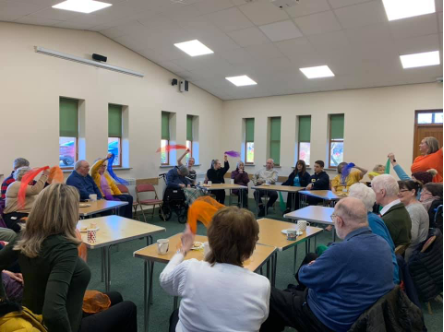
\includegraphics[width=.8\linewidth]{Images/ChapterFour/SilverlineCommunityRoomOne.png}
  \label{fig:communityRoomOne}
\end{subfigure}%
\begin{subfigure}{.5\textwidth}
  \centering
  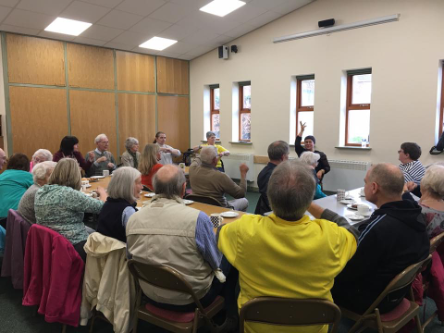
\includegraphics[width=.8\linewidth]{Images/ChapterFour/SilverlineMemoriesCommunityRoomTwo.png}
  \label{fig:communityRoomTwo}
\end{subfigure}
\caption{Silverline memories community room (taken from Silverline Memories Facebook)}
\label{fig:SilverlineCommunityRoom}
\end{figure}

 With the community room being shared across many different groups, Silverline memories had never had the chance to make space their own. Instead, you had a sense of 'home' or 'community' through the interactions with the volunteers and members. As I had set up the room, I got my notebook out, VR headset, and a recorder and consent/information sheets. As the first couple entered the café, Sandra and the other volunteers came over to them with open arms – similar for everyone who walked in on that day. They caught up, got them a cuppa tea and biscuits and got them sat down. Sandra was immediately welcoming and had created a space that focused less on the diagnosis and more on creating social interactions through creativity, music, entertainment and shared experiences. Sandra introduced the couple – Philip and Kate, to Kellie and I, and they were so appreciative and warm. They asked about the research, what we did, and showed such enthusiasm for why we were there. As I would find out in the study, the initial few minutes of signing consent, and reading information sheets and explaining the research are uncomfortable for all those involved. At that moment, it went from an informal conversation and into a formal study where two of us would be analysing and studying what was said. As we described the study, both were very happy with taking part in the conversation about the types of VR experiences they'd like to see. They were okay with quotes being used as long as they were anonymised. 

The workshop was my first experience working with people living with dementia, but more importantly, the first time I would be seen as a 'researcher'. Although looking young, and of course, getting sarcastic comments from the participants about my age and that I'm too young to be a researcher, I didn't know how to conduct myself in conversations with this new title. Each conversation felt like an interview, and there was a sense of power imbalance.  In some instances, power imbalance came from both sides, with members of Silverline Memories having been a part of the cafe for some time. Members didn't have to talk to us or take part in the study, and if they didn't, they had nothing to lose. On the other hand, Kellie and I were the only ones walking around with that title of 'researcher' who were here to interview and record participants. It was so unnatural to me, but why would it be natural? I don't start my conversations with friends or family with consent forms and placing an audio recorder on the table. Yet, the methodologies I was told to follow focused on the importance of researcher-participant relationships. 
 
From our conversation, I was surprised to see such common links with other papers I had read around HCI and dementia - people wanted an experience and 'fun' with the technology. Thomas wasn't interested if VR could help reduce care or anything focused on medicalisation, just how technology could be used as a form of entertainment. Thomas expressed Janet's passion for \textit{"listening to music and playing"} and that when she was younger, \textit{"she used to be in a choir... so it's been a big part of her"}. Regularly, the couple would explore YouTube videos looking for performances, which is why Thomas suggested a virtual theatre as he thought it'd be an \textit{"effective way of allowing her to experience something approaching live music once more"}. As our workshop ended, we had gained an overview of what may and may not work with the environments we would be creating. I then returned in a month with three different VR environments - a beach, park and a tailored Shania Twain concert hall for Janet and Thomas.
 
As I sat down writing, I felt a strain of being a 'researcher' or an 'outsider' in this perspective'. Akindes says that \textit{"through reflection, the meaning becomes visible in the process of writing"} \citep{akindes_pahalas_2001}. In this case, I'm talking about my privilege. As a white British male, I had never taken on any particular title that may place me as an 'outsider' throughout my entire life. Many of the members were warm and welcoming to myself, but I will always remain as an outsider to some degree. Although we share some aspects of experiences with all the members of Silverline Memories being from the UK, based on their stories and mine, they are drastically different. Throughout my life, I've remained in education and had the opportunity to go to university. At the same time, many of the participants I talked to discussed stories of their working-class upbringings that I had no perspective to draw upon. Therefore, I remain to question am I a good fit to research into the area of dementia. Christine Bryden discusses how by living with dementia\textit{ "[she] ha[s] complete member research status and can provide an insiders perspective"} \citep{bryden_challenging_2020}. However, while this gives Bryden an insider perspective to her own experiences and an understanding in the similarities that are present with a diagnosis with dementia, as ethnographers, \textit{"we are never fully outside or inside the "community"} \citep{naples2003feminism}. Naples argues that during research, \textit{"we negotiate and renegotiate our relationship to the community through particular and ongoing everyday interactions"} \citep{naples2003feminism}. Even if I had been part of Silverline Memories for numerous years, the addition of the 'research' title would have shifted my identity within the group. If we consider gender, race inequality, and class divisions as part of the outsider phenomenon, then we must acknowledge the \textit{"powerful role we play in shaping what can be seen"} \citep{naples2003feminism}. While as a researcher, we are not the only ones creating the academic knowledge nor can we control its effects, we must be aware that it plays an essential role during and after the research \citep{irwin_into_2006}. Whether we believe we have an outsider or an insider perspective, our research is to make changes to the research population, not ourselves. 

\section{Designing VR environments}
\label{Relationships:DesigningVR}
Over the next month of creating the VR experiences, I felt immense anxiety and stress about creating something interesting. Even though expectations may have been low from the participants, the pressure to make a well-researched project from my final year project and that I didn't want to let Sandra or the participants down was on my mind. Over that month, conversations with my Grandma consisted of sharing our experiences of dementia. While we had different understandings and experience, I realised the challenges she faced as a caregiver—mine from a research perspective and hers from a caring one. Pursuing dementia research not only was a personal endeavour from prior family history, but it also opened up conversations I had always been afraid to ask of my Grandma. Selfishly I know, but asking more about my Grandma's relationship with dementia, I thought, would give me a clearer perspective of how I may design for people living with dementia. I'm not sure if it did, but it gave me a sort of connection and empathetic feeling to the topic. I continued to be interested in the area, and during that time, I got to connect in a way to my Grandpa; I never thought I would have. Listening to my Grandma's stories about the challenges that came from his diagnosis influenced my perspective on dementia research.  The influence and relationship I have with my Grandma is a significant one in my research. While her stories painted a picture of their relationship that had its 'ups and downs', it was relatively a positive story of living with Alzheimer's. Over time, I began to realise and acknowledge that I overlooked the challenges and complexities that people with dementia may face - either the individual or carers. Only by spending more time in Silverline Memories – with other people living with dementia, would I gain a more in-depth understanding of the vastly different experiences people have had.  

With around four weeks to develop the VR environments, I enrolled in a VR online course by Udacity. With VR development being relatively new and not an area the university specialised in, I contacted the online course representative at Udacity to consider myself for a scholarship for their VR course. In early February, they got back to me and found the study of personalised VR for people living with dementia "innovative" and "novel" to the area. They sent me an online access code, and throughout February, I started to juggle learning VR game development with the rest of my university modules. The course gave me invaluable experience in building VR environments in Unity (a game engine). However, what it didn't describe was the importance of the particular placement of objects within the environment. For this project, I applied Mike Alger's \citep{alger_visual_2015} concept of content zones that I describe in fig.\ref{fig:ContentZone} that helped reduce risks of sickness or disorientation and improve the individuals' overall experience. Another limiting factor in deciding to use VR was anything that could create photo-realistic environments was expensive and bulky. Instead, I had to rely on taking a more stylised and abstract view of reality by exploring ways that low-poly art would portray the participants' desires.

\begin{figure}
\centering
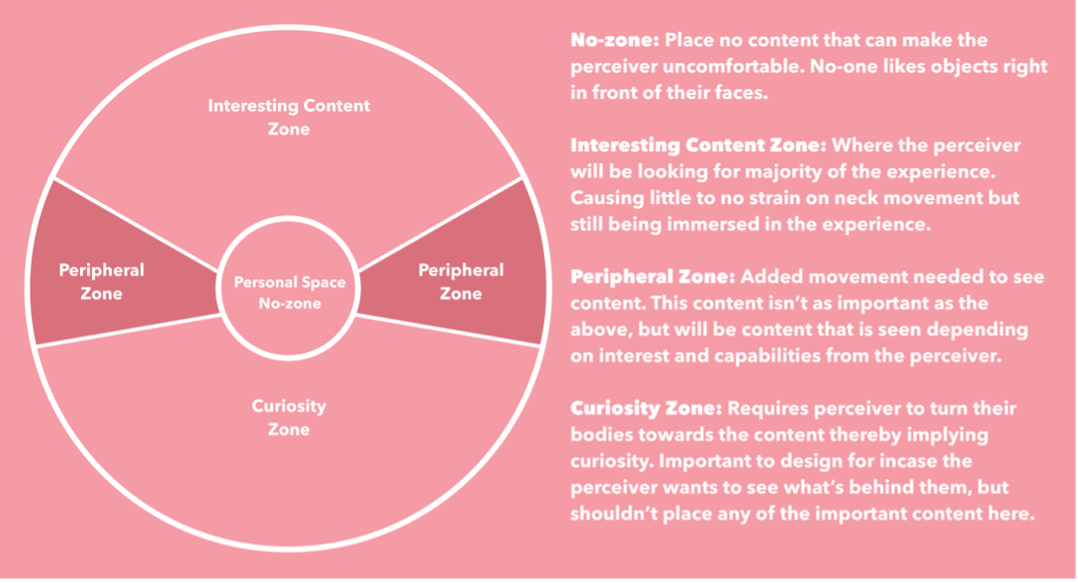
\includegraphics[width=.8\linewidth]{Images/ChapterFour/ContentZones.png}
\caption{Content zones in VR}
\label{fig:ContentZone}
\end{figure}

From the data collected from our first workshop, we created moodboards (shown above) based on the ideas and desires that individuals expressed. While we could not develop each participant's individual experience, participants' ideas were combined into one environment. For example, one participant asked for us to 'take [her] back to Ireland, to see the beautiful castles again'. While we couldn’t get any 360 footage from the castles the participant asks for, we did create 3D objects of a traditional castle from Irish medieval architecture. We placed it in the park environment that many participants expressed interest in (see Fig.\ref{fig:IrishCastle}).

\begin{figure}
\centering
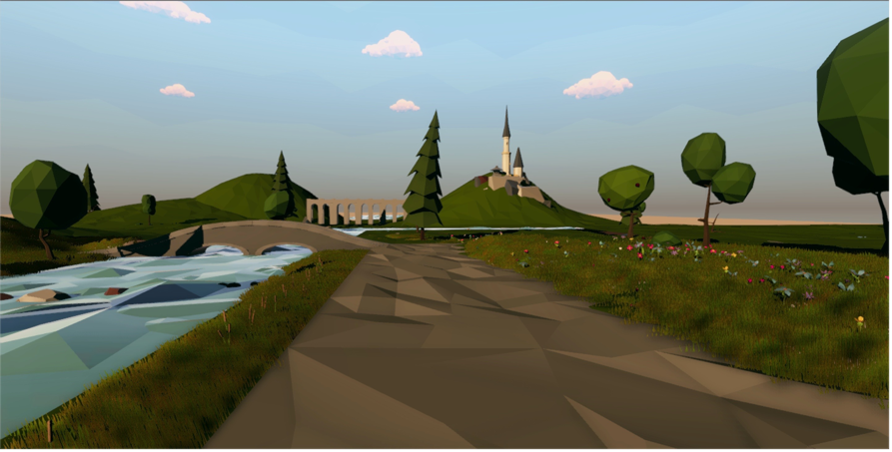
\includegraphics[width=.8\linewidth]{Images/ChapterFour/IrishCastlVR.png}
\caption{Park environment including an Irish castle}
\label{fig:IrishCastle}
\end{figure}

During the workshop, many participants expressed the particular environments of going to the beach or the park, following conversations of intricate details of Jesmond Dene Park or Whitley Bay Beach (both popular locations in the North East). Aspects would often resemble participants saying "I love the chirping of the birds", or explicitly remembering particular structural details such as "I love the bridges over the lake", and telling me stories of the Whitley Bay lighthouse. As I had written in my reflection in 2017, "I'm building a product to create positive experiences and potentially create some sort of reminiscence, I want to find those key objects that run through the [particular environment]". Back in 2017, reminiscence was a significant influence on the way the VR experiences had been designed. While, to some extent, they had an abstract style not to represent a particular location, adding in specific objects or sounds was done to provide familiar experiences for people living with dementia. While reminiscence has its promising evidence base and can provide opportunities of engagement, designing to attempt to 'cast back' to earlier positive moments may burden the person living with dementia by the past and relies on their perceived cognitive deficits. 

\begin{figure}
\centering
\begin{subfigure}{.5\textwidth}
  \centering
  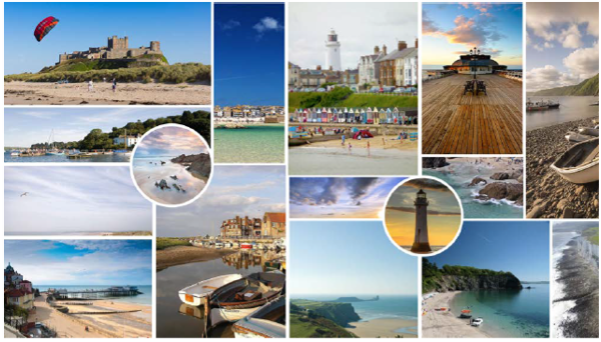
\includegraphics[width=.8\linewidth]{Images/ChapterFour/MoodboardOne.png}
  \label{fig:moodboardOne}
\end{subfigure}%
\begin{subfigure}{.5\textwidth}
  \centering
  
\includegraphics[width=.8\linewidth]{Images/ChapterFour/MoodboardTwo.png}
  \label{fig:moodboardTwo}
\end{subfigure}
\caption{Beach and park moodboards}
\label{fig:VRMoodboards}
\end{figure}

\section{Returning to Silverline Memories}
\label{Relationships:Returning}
A month later, I went back to Silverline Memories to conduct the second workshop. Given that the charity had recently won a lottery fund, the Monday session I held my workshop in was in parallel with their celebration activities. The celebration put less pressure on me, holding the room entertained. It's not surprising to anyone who has used VR before, but it's rarely a shared experience that would have caused difficulties when dealing with a room of 30 people. Fortunately, having the entertainment of a magician that was part of the ongoing celebrations and offering people to try the VR experiences ensured that everyone in the room was being entertained and not just waiting around for the VR experiences.

Multiple partners/carers tried the park and beach experiences and adored it. I remember thinking about how well the workshop was going but trying to think about how I can evaluate this? How can I say someone was emotionally happy or that they remembered something from the past? I didn't have any guidelines, but maybe that didn't matter. Surely my observations and the way I talk about it is enough? What I did know is this workshop felt very 'authentic'. I thought the workshop felt part of the dementia cafe this time around. I took the lead more in the research aspect, participants that we met a month ago asking how I've been and what I had been up to since the last visit. The research activity fits into the celebration, and people found the park and beach experiences beautiful.

As mentioned before, I had my doubts about VR not being interesting enough for the wider group, given it's a very isolating technology. During participants use of VR, participants and their caregivers expressed a wish to share in the same live VR experience as their partner or parent. Participants indicated that meaningful shared experiences with their loved ones with dementia had changed recently or decreased in frequency when asked about this. For example, Linda, whose husband Michael is living with dementia, mentioned that the couple no longer drove and used public transport. This meant that the two could not visit favoured locations together. So, they indicated that the VR park and beach could be used to supplement their recreational activities and allow them to experience a semblance of the sorts of activities that used to mean very much to them. Having the carers experience the environment first allowed carers to help direct their loved ones around the environment by probing specific interactions in the environment that the person living with dementia may have missed. For example, one carer started asking questions about what they could see or if they saw the horse walk past on the beach.

Near the end of the workshop, I sat down with Thomas and Janet to show them their personalised Shania Twain concert hall. With the current room where we were getting relatively loud, we asked them to sit down in the church attached to Silverline Memories. The room was more private with just Kellie, myself and Thomas and Janet. However, with the VR environment being personalised, and I had spent more time developing it only for the one couple, there were this expectation and pressure to make sure I captured the experience and data collection. Similar to other participants in the workshop, Thomas and Janet saw VR as a novelty and a technology that they had never had the opportunity to experience.

Janet's reactions to first trying VR echoed that of prior participants – with concern and uncertainty. As Janet started to hear Shania Twain singing, she began to \textit{'hmmm' }to the song and held the headset that Thomas was holding up for her. While Thomas has initial concerns with Janet having the \textit{"patience to hold the [headset] for a long time"}, Janet was engaged entirely through her body movement and was "\textit{start[ing] to sing. She was singing to the tune and attempted to repeat the lyrics"}. While I had a minimal conversation with Janet through the workshops as her verbal abilities are limited, other ways of communicating became apparent through the way she explored the VR experience. As Janet finished the 5-6-minute experience, she passed the headset back over to me and had a broad smile on her face gave us a wave goodbye. As we ended the workshop, the celebrations for Silverline didn't stop. As I was leaving, we said our goodbyes and I remember Janet looking back at me and giving me a big wave to say bye.

As I left, I didn't reflect that this was maybe the last time they'd experience the environments I had created. In my mind, I had developed some very rough prototypes that were prone to breaking. This holding onto the prototypes did create frustrations between Sandra and me over the continued relationships we had with Silverline Memories over the next couple of years.  These frustrations could have been from me not setting out clear expectations, or Sandra was expecting a lot from the project and having an 'app' that the dementia café could use. Over the past ten years, digital health apps have dominated technological solutionist approaches and mainly gained interest through the suggestion that with young people being 'tech-savvy', apps could connect particular populations \citep{byron_apps_2019}. 'AppMovement' is a platform that encourages collaborative design and development of mobile applications \citep{garbett_app_2016}. AppMovement gained popularity and has shown apps can be successful and valuable through developed apps such as FeedFinder \citep{balaam_feedfinder_2015} and Safe Places to fly your drone.
However, they rely on the uptake and participation of users, and they are designed in a particular manner. They may not necessarily be well suited for specific communities, such as people living with dementia. Sandra's expectation for a fully-fledged out app questions a sociotechnical knowledge barrier between us. With little to no resources and little time, an app was out of the question to have ever been developed.  Eventually, in 2019, I recreated the environments and gave them to Sandra alongside other objects and technology we developed through the ongoing collaboration. While it was not an 'app', it was workable prototypes of the three experiences. Towards the end of this chapter, I break down particular moments that created a complicated working relationship between myself and Sandra. Looking back, was it unethical to take away the experiences? The group never had the opportunity to try the experiences again. Of course, the time frame was concise, with it being an undergraduate dissertation. However, without learning from these ethical mistakes, I would have unlikely understood the importance of what defines 'impact' or 'legacy' of the relationships and technology you create in socially-oriented research. 

\section{Understanding researcher-participant relationships}
\label{Relationships:researcherParticipant}

Through the first six months of my Digital Civics MRes, I had the opportunity to learn about a range of topics and areas of research that seemed foreign to me during my undergraduate. From learning qualitative research methods to how, as researchers, we can engage in socially-oriented approaches. A core part of Digital Civics is \textit{"how our digital research could be of use and value to local councils and local citizens"} \citep{olivier_digital_2015}. To some extent, I had done a similar take on my undergraduate research when working with Silverline Memories. A key theme through learning about Digital Civics was the idea of 'empowerment'. How do you design to empower the citizens that use the technology? With Open Lab being a leading HCI lab in the field, particular examples of Digital Civics created spaces for both citizens and local government through digital participatory platforms such as 'App Movement' \citep{garbett_app_2016} and 'Make Place' \citep{peacock_streets_2018}. Similarly, in a less socio-technical perspective, a determination by governments and Alzheimer's societies promote dementia-friendly communities that bring groups of people living with dementia to influence services and policies or create spaces to share experiences or to have a place that is rid of the societal complexities that someone living with dementia may experience with a diagnosis. In 2017, Morrissey et al. explored an app created through App Movement called 'Care and Connect' to identify and rate public spaces on their 'dementia friendliness' \citep{morrissey_care_2017}. The study reported that while people living with dementia were \textit{"interested and comfortable in using the app, it is mostly used by carers at the moment"}. Of course, App Movement was not specifically designed for any particular community but demonstrated that members of the community wanted to meaningfully express their thoughts and to be involved on a level that saw fit to their desired engagement.

In a similar fashion, although people living with dementia have been involved in planning, decisions and discussions of 'dementia-friendly communities', Swaffer reports that in the UK, approximately 350 people with dementia had been directly engaged in the work… that is an unacceptably low number" \citep{swaffer_dementia_2014}. A lack of involvement of people living with dementia contributes to the stigma and discrimination within society. While we have seen recent research in HCI and gerontology research into the area place significant importance in engaging with people living with dementia, the extent to which we involve people living with dementia and the implications remains a contested and under-examined issue. As a community of researchers, we should be echoing similarities in the Dementia Enquirers group that are developing new design approaches to research led by people living with dementia \citep{diaries_deep_2020}. By involving the community during grant stages, identifying research priorities, and planning research, we can ensure research agendas are more closely aligned to the needs of that given community. While I must admit, I have not achieved in full the scope of what I have discussed above. Still, as I moved from my undergraduate where I designed for people living with dementia, in the study that follows, I move a step further by considering ways we engage with not only the person living with dementia but working closely with families to co-plan days out, and to facilitate active participation through the study. While I was reading up on the breadth of literature around involving families and carers in dementia care, the same attributes of relationship-centred care can be followed in how we should engage families living with dementia in HCI research:
\begin{quote}
Good communication will contribute to a good-quality relationship by helping each party to understand the other party's perspective and enabling differences to be discussed and, where possible, resolved. It will be respectful, recognising the expertise of the family member and that each party has much to learn from the other. A good relationship will improve the quality of care, by helping relatives to act in an advocacy role for the resident, and by ensuring that the important information that the relative has (which can make such a difference to the individualisation and personalisation of care) is shared with those staff involved in hands-on care. \citep{keady_involving_2007}
\end{quote}

Keady et al. highlight the benefits of involving the person living with dementia and their relatives and care home team. Although each situation of working with people living with dementia is individualistic, the emotional 'burden', guilt, and overwhelming feelings that those around the person living with dementia may be feeling, should be considered and explored. To continue and build from the prior VR exploration, I worked with Silverline Memories to work with three families who explored how they could capture meaningful experiences using photography, audio recordings, and more contemporary technologies such as 360-degree video cameras support families living with dementia.

Reflecting on what didn't work and what did in my undergraduate research, I wanted to focus on three differences to the prior work: 1) designing for moments, not memory, 2) insider-outsider relationship, and 3) the act of giving. My first point – designing for moments, not memory, is a move away from designing for reminiscence and considers the philosophy of \textit{"[if] the present is all that person has, [then] that is their reality"} that Silverline Memories support group follows \citep{hodge_exploring_2018}. While the VR experiences had an art style that enacted as ambiguity and created space for people to reminisce on their own lived experiences of beaches, and parks, through developing the three environments, my design approach was to represent participants memories through the environments such as one participant asking to \textit{"take [her] back to Ireland, to see the beautiful castles again"}. While reminiscence was apparent and effective in the study, I began to question if relying on the person's ability to recognise or articulate past events is an appropriate activity to enhance emotional connection \citep{lazar_systematic_2014}. Another notable concern I had was the tensions that arise from the insider-outsider relationship. Through the workshops, I initially got to know some of the members of Silverline Memories, but there was a strong presence of 'researcher' title and power imbalances, and perhaps they always will be. I'm still going to be the 'researcher', and I am researching them, but how can I improve this? Researching under a culture of ethical 'protectionism' already caused significant tensions about formally acknowledging participants as co-creators, I sought to recognise and acknowledge participants as individuals who will contribute to the research and ensure that their knowledge, experiences and time are appreciated through compensation that is meaningful to the participants.

Furthermore, compensation leads to the act of giving. The exploration of VR experiences resulted in three prototypes that were never developed for continued use or different hardware while positively appreciated. This caused tension in the relationship between Sandra and I, which I didn't want to happen again. Instead, the study with the families would present the members as co-creators who would be working towards developing a final product for them. I wanted to ensure that the families felt appreciated and that the 'meaningful experiences' they created on the days out would be in their hands forever. I hoped this would acknowledge and appreciate the time and effort they would put into the research and be a way to consider the 'ending' of the project ethically.

Working with Silverline Memories again, I went to one of their activity days to ask families if they would like to be involved in the study. Each family would engage in a piece of research through design (RTD) \citep{zimmerman_research_2007} work to explore the opportunities and challenges of designing enriched personalised multimedia experiences. The families would choose a 'day out' where we would go and capture meaningful moments through photography, audio and 360-degree videos that were to be deployed in VR headsets. After their days out, families would be invited to a series of design workshops, whereby families would work with researchers and designers to curate personalised media experiences from their meaningful moments. As I arrived, Sandra welcomed me back again and was looking forward to working together still. Unaware of this, Sandra said I'd be running the Silverline Memories session for the entire group. Remarkably unprepared and put on the spot, I felt expected to do what Sandra was asking. Sanghera et al. discusses the relationship between the 'gatekeeper' and researcher, is an important one, "yet it is a relationship that is fraught with inconsistencies and instabilities" \cite{sanghera_methodological_2008}. Crucially, gatekeepers have control over who is recruited and the refusal of participation. While Sandra, cannot refuse permission for members of Silverline to be recruited, information about the study went through Sandra which she could withhold. Arguably this relationship is important one to keep reciprocal to ensure access within the community. Furthermore, Coffey argue through the study: researchers, participants and gatekeepers have their own interests and needs and are likely to differ from one another. Expectations can be perceived clearly or implicitly through research, and in my own work, I perhaps didn't reciprocate Sandra's needs or expectations in the right manner. 

As I discussed in the prior sub-chapter, it took two years for Sandra to get the VR experiences with a fault on my part. Still, throughout these years, I had placed significantly more time on respecting the interests of the participants as opposed to Sandra's. What I failed to recognise was Sandra wanting me to volunteer and support Silverline Memories. Researchers who work with non-profit organisations (NPO's), may get emails or texts asking to help run activity sessions, and in turn, the research acts as a volunteer instead of being a research. Researchers who have experience in sensitive settings or have committed time in a marginalised community have invaluable skills for NPO's.  In more deprived areas, non-profit organisations (NPO's) tend to have an abundance of skills, volunteers, and cash. Marshall et al. discuss findings of volunteer effort to be not only preferred compared to donations but that its \textit{"important from a funding standpoint"} \citep{marshall_accountable_2016}. NPO's ability to quantify the number of volunteers and how they contribute to research studies, can be seen as an invaluable addition to their NPO. The difficulty from my work was a miscommunication between Sandra and me. The research was focusing on the families and not necessarily to benefit Silverline Memories. However, looking back, navigating how my time could have helped Sandra by volunteering, writing blogs about Silverline Memories partnership with Newcastle University would have benefitted the relationship more than creating replicas of what was created for the families for Sandra. Going through a gatekeeper among the challenges of relying on level reciprocity also led to potential ethical challenges. Sandra, as the gatekeeper between the researcher and the Silverline members, Sandra had the opportunity to control who I spoke to and who I may conduct research with. While I believe Sandra suggested the particular families that ended up being participants was for my benefit and not hers, the control split the members towards those who may be 'good' fits for the research and those who may not create 'interesting' or 'useful' research findings that Sandra foresees.  

Through the project, I wanted to work with at least two families but on a more intermediate level compared to the previous study. Sandra had recommended that Kate and Philip take part in the research, but another family or two families that Sandra suggested were Lauren, Michael, and Sarah and John. Both couples had recently joined Silverline Memories and created a bond between one another. Sarah and Lauren were both diagnosed with dementia about two-three years ago. Through the relational context, Michael and John bonded over particular situations and over time, so have Sarah and Lauren. As I approached the four and introduced myself and why I was here at the dementia café, Michael seemed somewhat sceptical of my reasons and the research. He initially started to make jokes about am I going to "spy on them", or that I "look awfully young to be a researcher". At the time, their jokes were on the line of them trying to be defensive and welcoming that I was around them. My identity was being challenged, and, at this moment, I had to \textit{"prove that [I was] worth of their time"}. It isn't that often that many members of Silverline get to take part in research, and for some of them, the attention from outsiders is remarkably welcomed. I don't necessarily fit into the space that the families or members co-exist in. What I'm doing is maybe obscure to them. I'm not necessarily supporting care, and I have a lack of lived experiences to pull from – which is apparent from comments about my age. As soon as they saw me, they knew I wasn't apart of Silverline Memories or that I was not a volunteer either. We got talking, and both couples wanted to take part in the study as a group. Michael and John took the lead on where the group would like to go, and they decided on a national trust park in Northumberland.

A few weeks later from the initial recruitment process, I picked up Michael, John, Sarah, and Lauren, excited and ready to go on their day out. The families filled in the consent forms, and it went pretty smoothly, even if it did make the start of the day a little awkward. Lauren and Sarah both can still read and write, so they signed their consent sheets, and we went on our way. Throughout the day, I had a set of semi-structured interview questions to ask the family. Given the nature of the day out being co-designed by the family, and that they decided on what to do throughout the day, the questions came out very naturally in conversation. Through particular discussions with each member, I was able to drive the conversation into specific questions.  For Michael, the day out allowed him to let his guard down his caring duties and socialise with others. Quite often, Michael would be asking about my life and telling me stories of his past – less about his current situation and more conversation around non-dementia related topics. He found solace in this, to the extent that later through the study, he told me \textit{"this felt very much like therapy. Thank you so much for listening"}. However, particularly with Michael and Keith, they would often share stories of challenging encounters they have had while caring for their partner. They would then reiterate sayings similar to \textit{"is that the type of things you want us to talk about?"} or "\textit{would x be useful for the study?"}. Wang echoes problems with the authenticity of qualitative data that may occur in researcher-researcher relationships \citep{wang_construction_2013}. Similar to Michael and Keith, Wang discusses students who would 'act' differently and emphasise particular moments by saying "you should write this down in your report". On these occasions, I wondered at what point are these conversations not only 'valid' in my analysis, but with some conversations being particularly open and to some extent, over-sharing, where is the line drawn? Michael was very aware that he would be recorded throughout the day, but during the spur of the moment conversations, would he want some of the topics of guilt, grief and his internal struggles be published in publications, or was it more a call for help.

Thinking back to the day, the change in tone from the families was noticeably different from what it was when I first met them. As we sat down for lunch, Michael commented on the 'change' in what he thought of me. At first, he thought I was relatively 'shy', while now he saw me more confidently. The comments from other participants that align with my personality, character, or even referring to the research title such as Michael saying 'are you going to be spying on us', they are comments that still bother me. Not because I'm offended or felt 'picked on', but because I wondered why were these comments made? Similarly, Rose et al. discuss during an interview, "another worker at the centre, walked past us, he laughed and said, \textit{"'look, I'm being interviewed for Radio 4'"} \citep{rose_situating_1997}. Rose again, is bothered by the comments but reasons of the uncertainty of what do the comments represent. In parallel to Rose, I wondered if these comments a reference to my note-pad with scribbled down notes alongside my audio recorder? Maybe it's a comment of my 'shyness' because I'm not acting like myself under the representation of a 'researcher' for Newcastle University – Am I representing a different version of myself?  I found that there is a lot of uncertainty in what participants say and that it's difficult to position ourselves in these particular ambiguous situations. While reflecting on these particular moments, I questioned how I could answer comments that are so uncertain in the analysis. But perhaps, not every quote or 'data' has to be analysed to understand its meaning. Again, returning to Rose' work on personality, and situated knowledge, as researchers we should \textit{"inscribe into our research practices some absences and fallibilities"} \citep{rose_situating_1997}, and through discussing to some extent, a failure in how to analyse this uncertainty in my position through the comments of the participants, perhaps by sharing these particular accounts, contribute to the overall narrative of other well-defined analytical pieces through this written account of the past three years.

Another narrative that has been discussed very little in my prior publications is the second family that went on the days out. Kate, Philip and their two daughters were invited to go to Seahouses – a particular Beach that held a place in the family's history. On the arrival of the planned day out, we went over the initial consent and information sheet details. As each family member signed and consented, we got to Philip. Philip, who is rarely verbal, and can no longer read or write, had some difficulties in partaking to the institutional ethics I had to follow. Despite the growing literature of people living with dementia participating in research, many researchers have accounted for moments where they had to exclude particular people from satisfying the ethical review boards processes. The makeup of an ethical review board (ERB) often consists of other academics who are unlikely to have experience in your field – and this can lead to a biomedical view. ERB's will try their best to have varying experience in particular areas. Still, due to the specialisation of research, it is not always possible to have a committee with expertise in dementia from both a person-centred and design angle. Based on my ethics approval I had gained for the study, I knew if any participant couldn't at least verbally communicate consent, then they could no longer be part of the study.

Consequently, I had an option to either walk away or continue with the day out but not count this as research. It felt unfair to walk away, and I would be contributing to that of older people living with dementia being excluded from being involved in research. While I couldn't continue with Philip being a participant, the day out was already set up. It would be morally wrong not to 'give' back to the family who had already spent time invested in pre-study preparations.

To my surprise, I had a sense of relief and my anxiety of conducting the research had gone. I no longer felt this pressure to attain 'interesting data' or apply the ethical principles that controlled, corrected, and structured the research. Of course, with the family signing up to take part in an RTD approach where they would get something at the end that expressed the meaningful experiences they created, we still took pictures, and videos during our day out, but it was vastly different. No more did I feel the need to place a recorder on every table where I sat down with the family, I wasn't overthinking every word that came out of my mouth, or how this will apply to my analysis. This echoes Irwin, who describes ending an ethnography of a tattoo shop where one of the participants became her ex-boyfriend \citep{irwin_into_2006}. To her surprise, she found comfort in moving her identity of being a researcher, to a friend of those she had become close to through the research. To Irwin, letting events naturally evolve paralleled the feeling of 'authenticity' that had been discussed by other feminist researchers who had tensions arise where their commitment split between the research participants wants and their research goals. As the day went by, Philips interaction between all of us radically changed. After we took a break at the local Fish and Chip shop, Kate commented on that she was "shocked at how much Philip had ate today… I've been struggling to get him to eat over the past few days". On our return journey Philip started to tickle his daughters' necks who were in the seats in front of him. He even prodded me in the side to amuse me and we all started to laugh. He turned to look at Kate and said "I love you". These acts from Philip that Kate and his daughters rarely had seen over the past year and cherished every second of them. Since my interactions with the family, I've been continuously frustrated with following the ethical principles in place. Philip could only consent at the start of the project, and in particular with that consent – it was cognitively informed. Dewing discusses a method for consent that is ongoing. It enables more significant and meaningful involvement from participants who may otherwise have been excluded from studies similar to mine \citep{dewing_participatory_2007}. As I write this and reflect back on experiences, my interactions with the ERB were rather limited. If I could have sought support, advice and had a more open collaboration through the ethical process, perhaps Philip's involvement in the research would have changed radically.

As I had finished the days out, and captured content with the families, I ran individual workshops with each family as a way to consolidate the personalisation and storing of the created moments from their days out. In the workshop, we shared pictures of VR videos in each workshop to give participants a perspective of the day out and to see the digital moments they had co-created. The families discussed how moments could be translated into technological media to be relieved or experiences with others. I shared some of the videos and images to the participants in the workshop and we iterated numerous ideas of how the families wanted to be able to access, experience and display their moments they captured. With deadlines being accounted for, once I had finished the workshops I had very little time to create any of the media experiences for the families for either my MRes deadline or the CHI deadline. Through my conduction of my analysis of the days out, it was apparent this would heavily side on Sarah, Lauren, Michael and John with not being able to gain consent from Philip in the other family day out. The analysis delved deeply into the idea of experiences of being in the moment as opposed to designing for reminiscence. Through this, it raised questions of in particular Michael and Laurens relationship. In many instances, Michael expressed frustrations of Lauren no longer having the capacity to reminisce a particular history of their lives, which brought him great grief. In my CHI publication about this study, I use many examples of the challenges that arised between Lauren and Michael to present the idea of how we design for \textit{'eclipsing realities'} \citep{hodge_exploring_2018}. At the start of the subchapter, I discussed how community members should be part of the entire process of the research and while I think that may be true, I imagine if I had done that with involving Michael and Lauren in paper writing or even giving them the opportunity to review the paper, the relationships may have turned sour. Returning to Wang, who discusses a participant who disagreed with the way she was portrayed in Wang's work. Wang battles with this dilemma in that \textit{"If I followed her suggestion to reconstruct the image that she had of herself, my research would lose its critical edge, and I might become a 'mouthpiece'"} \citep{wang_construction_2013}. My fear of sharing the paper to Michael portrayed similar dilemmas that Wang had faced. While I didn't hide the publication from any of my participants, as when I offered the paper to them, all participants shrugged it off and state they aren't bothered in reading the paper. As I look back, should have I been more open about what I was writing about in my work with the participants? Would they understand that the analysis isn't aimed at questioning the participants care or relationship, would they understand this when reading quotes of their interactions, but also, as the researcher, am I contributing to the exclusion of the community in research that I have discussed through my work.  

\section{Relationships that were forgotten}
\label{Relationships:forgotten}
I officially started my PhD in September 2019 and found myself surrounded by many other tasks that took most of my time, delaying finishing the prior project. By leaving the field with little to no repercussions, researchers can leave the study behind and return to their academic position \citep{abulughod_can_1990, gottfried_beyond_2016, irwin_into_2006}. Researchers get to continue their academic lives through conferences, presenting work, planning and conducting new studies. This privilege represented clear power distinctions between researchers and participants, particularly between researchers and caregivers who cannot leave if the caring role becomes too heavy. Irwin shares insights into her complexities of research relationships when they are attempted to be carried on after the end of the fieldwork. While my study didn't end after the workshops, the finishing of the moment boxes continued to be delayed creating frustrations by the participants as they would occasionally text saying \textit{"hope you haven't forgot us lol."}, or \textit{"are we still going to be getting the boxes?"}. The participants had been promised something and didn't want to feel led on. Despite my dedication to other projects, I attempted to keep the families up-to date with what was going on. With my original date of delivering the research through design prototypes to the families by Christmas not being possible, I sent personalised Christmas cards with photos and a photo frame with the group family pictures. 
 

\begin{figure}
\centering
\includegraphics[width=.8\linewidth]{Images/ChapterFour/FamilyPhoto.png}
\caption{Framed family photo}
\label{fig:familyPhoto}
\end{figure}

During the time away from the families, particular comments from Michael stuck with me. He would pull me to the side and express his gratitude for being part of the study and post workshop - \textit{"Thank you so much… this felt very much like therapy to me"}. During the workshop, he opened up a lot about his struggles with the different realities Lauren would be co-existing through. Michael's comments could be seen as a cry for help and the appreciation of being involved in the study calls to the considerable societal challenges associated with living with dementia. Swaffer expresses people living with dementia "\textit{want to access services and to participate in the community the way everyone has a right to expect, and to have our disabilities respected with acceptance, support and enablement"} \citep{swaffer_dementia_2014}. By taking a more person-centred approach to the study by including and respecting the participants' desires by co-planning where the research would take place, the research involvement promoted a more inclusive space and meaningful engagement for the families. 
 
\section{Designing the Moment Boxes}
\label{Relationships:MomentBoxes}
From the days out, workshops and analysis, the boxes represented each participant's desires and needs instead of focusing on the individual living with dementia. The final version of the moment boxes was developed in late March, with families receiving in early April. Design choices took influence from ways for realities to eclipse one another, to honour the individual's choice, and nurture caring relationships that are outside of the caregiver and care receiver's relationship. Each moment box came with an Oculus Go Virtual Reality headset, a personalised wooden picture box, and a bamboo wooden box filled with physical objects from the days out, or specific requests from the participants such as the dioramas.
 
\begin{figure}
\centering
\includegraphics[width=.8\linewidth]{Images/ChapterFour/MomentBoxespng.png}
\caption{Moment box}
\label{fig:MomentBoxes}
\end{figure}

 
\subsection{Designing for eclipsing realities}
\label{momentBoxes:realities}
During our days out, it became apparent that the person living with dementia may slip in and out of realities which could be contested by those around them, who may struggle with these conflicting accounts of reality. In particular, Michael expressed his struggle to orient his wife, Lauren, to reality. Michael shared a repeating act of telling Lauren her mother had passed away and would be coming over to see her. While this may place Lauren into the reality Michael sees, we must question if this is an effective way of care. When one cannot recall and recount memories, we should consider other ways to eclipse realities briefly rather than conflict with each other entirely. To do so, we may consider the use of lying or being deceptive as a way to eclipse one another's realities. Unsurprisingly, therapeutic lying is somewhat questioned in what context it is being used \citep{elvish_lying_2010, lorey_fake_2019}. Some researchers suggest that by lying, there becomes a sense of dishonesty, and once occurs, trust is broken, which significantly moves away from person-centred approaches. While it's easy to engage in debates concerning what is morally wrong, many researchers are not the ones dealing with the challenging situations in care. Lying and orienting the person living with dementia towards the 'right reality' will remain controversial, but it comes entirely down to the situatedness of the moment. With this in mind, in the design of the moment boxes, I considered ways the media experiences could be shared and experienced in multiple ways by considering each individuals desire, wants and possible levels of engagement.
 
Using 360-degree video capture meant that when the user would be playing it back, they would be the focal point driving along with the experience in all its richness. By placing the user as the centre of the moment they had captured, the 360 experiences could be interpreted in different ways. For some, the moments would be less about revisiting past, and instead foster emotional connections of the beautiful scenery in the video. Accompanied in the moment boxes, I placed tactile, scented artefacts, such as pine cones taken from the forest on the days out. While the families directed myself to take the videos and photographs through the day, by capturing the entirety of the space in 360 degrees, it means for Michael, he can watch and reminisce on these particular moments and watch as the family walk by the cameras and explore the national trust park, while for Lauren her gaze may focus on the trees, the birds, and flowers that were captured that surrounded the space instead. In the example below, we have Michael, Lauren, Sarah and John walking through the National Trust Gardens, where the viewer is given freedom to focus on the flowers and scenery, or the family.
 
\begin{figure}
\centering
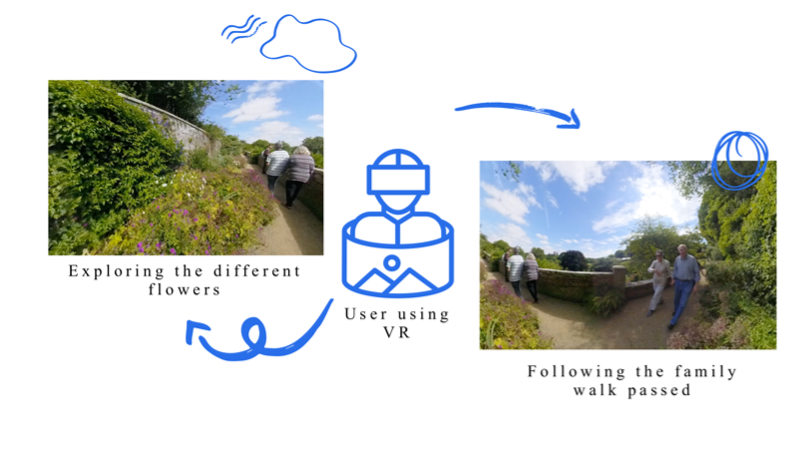
\includegraphics[width=.8\linewidth]{Images/ChapterFour/WaysToViewCapturedFootage.png}
\caption{Different ways to view the captured footage}
\label{fig:capturedFootage}
\end{figure}

For Philip and Kate, their daughters expressed they wish they could capture further meaningful moments for the family. Kate and Philip would spend time on evenings looking over images and videos that the daughters posted and shared on Facebook. Aligned with Philips interactions on the day out, his experiences and interactions strongly rely on the family that surrounds him, and demonstrates an importance of designing for supported family moments. In our moment box for Philip and Kates family, we created a set of tutorial guides to create 360-degree videos for their family gatherings. The tutorial explains how the families can place the videos on YouTube and create QR codes, which individuals can scan onto their phone and place into a VR cardboard headset to share and experience their 360-degree video moments. While I must stress that the use of media experiences is no substitute for going outside, or to replace nature walks, gardening with virtual reality versions, we must consider that these experiences are alternatives for engagement and immersion when the person decides not to go outside – or in a situation particular to as I'm writing this thesis, during periods when social isolation is a priority for all and social interaction is limited.

** Print out tutorial guide and take picture – Post Covid **

\subsection{Honouring the individual's choice}
\label{momentBoxes:IndividualChoice}
Nolan et al. argue that people living with dementia have reported a lack of confidence when going out \citep{nolan_perceptions_2006}. As we age, our cognitive abilities are likely to change. By creating opportunities to communicate oneself, such as getting their hair done, dancing, and choosing the way to dress, we start to consider how we honour the individual's choice in respectful ways that represent their personhood and individuality \citep{twigg_dress_2013}. Through the days out, I got to know the families and some participants were more explicit than others. Michael expressed his needs such as asking for a VR guided experience. But for Lauren, it was apparent that at times, Lauren would lack a sense of individuality. As we followed the larger group, Lauren said: 

\begin{quote}
    
\textbf{Lauren:} "You take note because I forget which way I come from, where I'm going to."

\textbf{Researcher:} "Don't worry. No problem. if we get lost, we'll get lost together. That's fine. It's so beautiful. You've been here quite a few times, Is that right?"

\textbf{Lauren:} "Yes, Yes."
\end{quote}

Throughout getting to know Lauren, her expressions ranged from moments of anxiety similar to above to confident chat about hobbies and interests, from wildlife to the carefully modelled miniature figurines she admired in the national trust site. To honour Lauren's choices and preferences, I created a set of personalised Dioramas placed in the top-tier section of the moment box (see fig.\ref{fig:Dioramas}). The Dioramas are inspired by particular locations we spent significant time at Wallington National Trust, and yet they remain abstract enough to be enjoyed by others.


\begin{figure}
\centering
\begin{subfigure}{.5\textwidth}
  \centering
  \includegraphics[width=.8\linewidth]{Images/ChapterFour/Diorama1.png}
  \label{fig:DiroamaOne}
\end{subfigure}%
\begin{subfigure}{.5\textwidth}
  \centering
  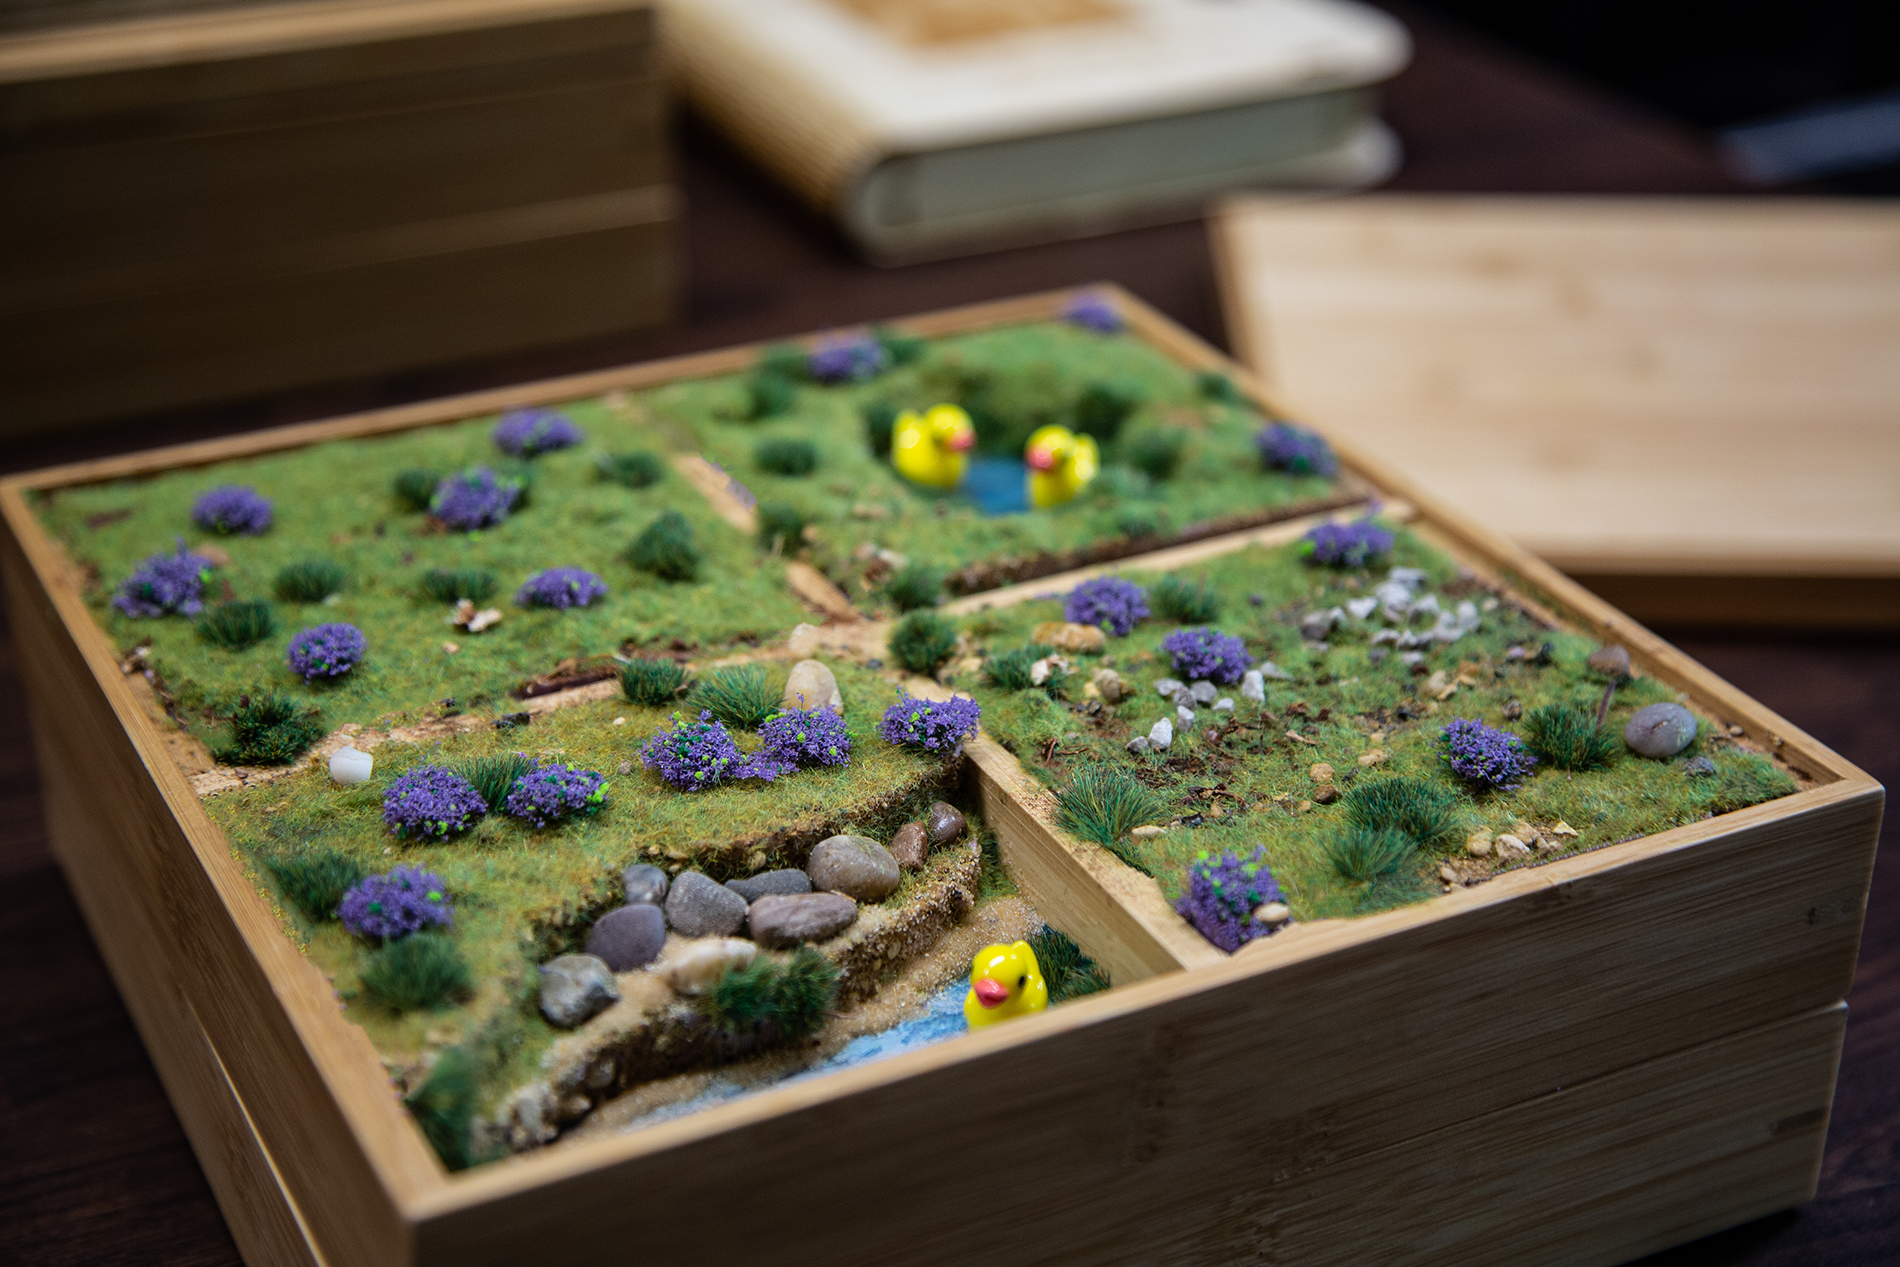
\includegraphics[width=.8\linewidth]{Images/ChapterFour/Diroama2.png}
  \label{fig:DiroamaTwo}
\end{subfigure}
\caption{Dioramas created for Lauren and Sarah}
\label{fig:Dioramas}
\end{figure}

To honour the relationships between different family members, Sarah and Lauren's relationship became evident through our interactions and conversations. Michael recalled their family holiday with the four of them, and Michael mentioned that Lauren and Sarah \textit{"walked up the seafront hand in hand all the time chatting away"}. In designing for their relationship, each of them got a set of 'Lauren and Sarah's moment's which was particular snippets of videos of the two together and photos that are focused on their relationship solely.

Family members also expressed the types of material for the moment boxes. Through a couple of iterations and engagement with family members, bamboo was decided to be light and sturdy for the box. While this limited the customisability that the cardboard boxes offered, they remained sturdier and would last longer. In one of the workshops, Kate shared \textit{"Philip likes to pick at things or pull at corners of card…I think the boxes would have to be wooden or made out of something more solid so it can last longer"}. With more time, I could have perhaps created a more personalised box with a custom-made handle and lock on the sides to make the item more portable. Still, given the time frame and overdue handing the boxes over to the families, I had to sacrifice particular design decisions.

\subsection{Nurturing caring relationships}
\label{momentBoxes:caringRelationships}
From early on, I aimed to design the media experiences with not only the person living with dementia, but to include their family members and friends. Traditionally, studies often separate carers and people living with dementia as previous work expected different needs from one another. When carers are designed for/with, technologies typically have a focus on duties of care with direction towards assistive technology  \citep{bennett_assistive_2017, bharucha2009intelligent,gibson2015everyday}. Spending time with the ecology of care, and with a focus on memorable and pleasurable activities, the overall technology or activity tends to include a variety of interests and interactions that the ecology of care desire. With many carers reporting high levels of burnout and burden \citep{takai_experience_2009}, targeting carers as research participants worthy of digital interventions focusing on personhood (as much as we target those with dementia) means treating them with respect, and as whole persons, rather than defining them by their roles. 

As discussed before, Michael wanted to share experiences that would place Lauren in experiences that required to articulate past events as their history held significant importance to him. For this reason, our 360-degree experiences tailored for them can also be used on a phone or tablet. With some ambiguity in what families exactly wanted in how to access the experiences and given their recent introduction to VR technology, I created multiple ways for families to explore the media experiences they captured. The first, was a ‘walkthrough’ experience where the user can navigate to different areas of their day out by clicking on pink circles on the video (see fig\ref{fig:wallingtonTrust}). For example, clicking ‘Walk to the Chinese Pond’ from the entrance video will take you to the Chinese Pond video. For Michael, the video walkthrough gave him the ability to explore the estate and history through the day out and for him to be able to express his experiences through recognition, if Lauren chooses to do so, she can join the experience through the same exploration too. 

\begin{figure}
\centering
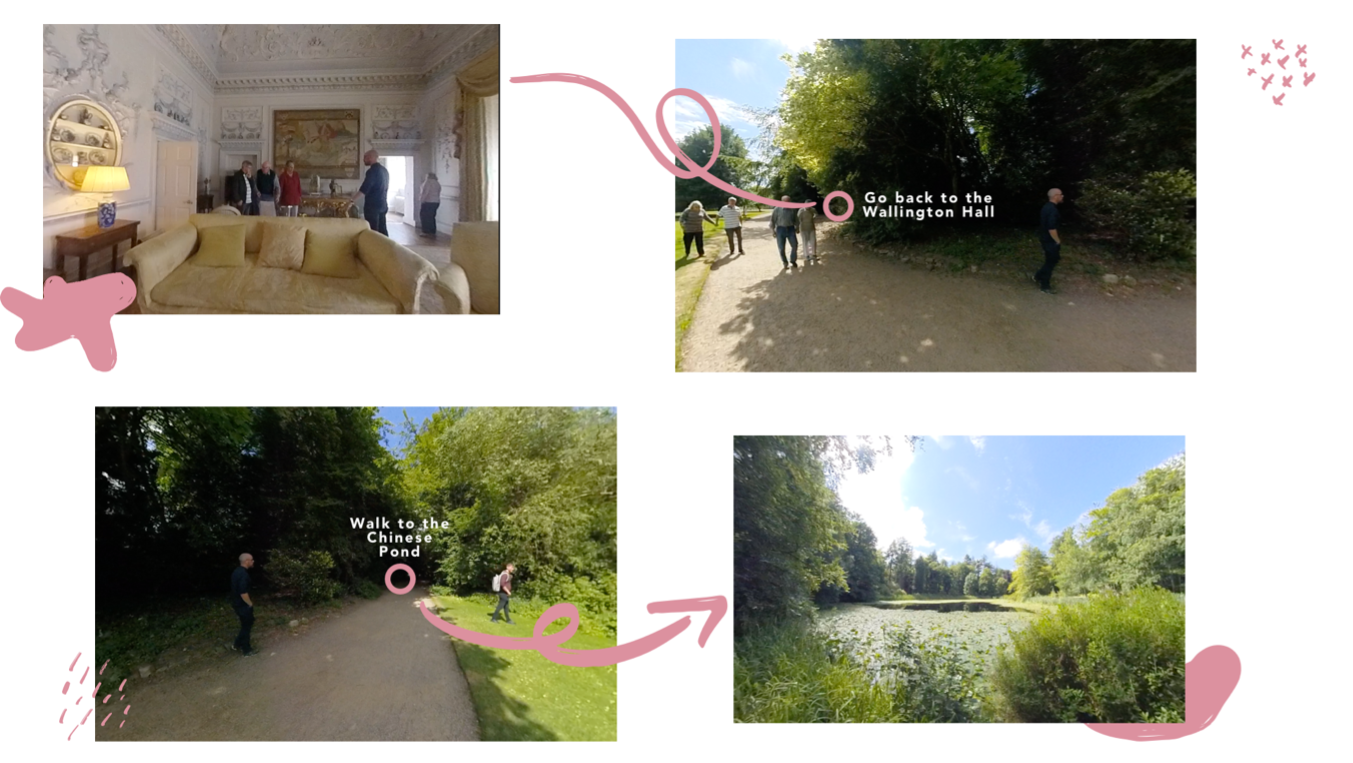
\includegraphics[width=.8\linewidth]{Images/ChapterFour/WalktrhoughOfWallington.png}
\caption{Walkthrough experience of Wallington Trust}
\label{fig:wallingtonTrust}
\end{figure}

Our second way to explore the day outs was to create an activity that Lauren, and Sarah to take part in and potentially with others from the dementia friendly communities they are a part of. The experience attempts to encourage shared, meaningful interactions. Through a set of ‘random’ QR codes, users would select a QR code that resembled a random moment that the family captured on the day out. Users then place it into the square (shown in fig.\ref{fig:QRcodes} and scan the QR code on their tablet, or phone – which in turn, would open the video up onto their phone.

\begin{figure}
\centering
\begin{subfigure}{.5\textwidth}
  \centering
  \includegraphics[width=.8\linewidth]{Images/ChapterFour/InsideQRCode.jpg}
  \label{fig:insideQRBox}
\end{subfigure}%
\begin{subfigure}{.5\textwidth}
  \centering
  \includegraphics[width=.8\linewidth]{Images/ChapterFour/QRCode.jpg}
  \label{fig:QRCode}
\end{subfigure}
\caption{QR codes VR activity}
\label{fig:QRcodes}
\end{figure}

This interaction while could be used between any of the couples who took part in the study, I wanted to create a way to interact with the experiences that could not be influenced by other people’s needs. With the ambiguity of the QR codes, the choice of the moment was selected by random by whoever decided to pick up the QR square from the box. As the media is designed for shared experiences, this leaves it open as an experience that both partners can interact with solely, as a couple, or together with other loved ones to enrich their lives and provide comfortable, evocative experiences. Finally, families expressed share their experiences with others such as other family members who did not have the chance to get part in the day out. Through Vimeo, I curated a showcase with an archive of all the videos taken from the days out (see fig.\ref{fig:onlineArchive}). In the boxes, I printed out multiple different small cards that families could share with others with a bit.ly link for others to watch the videos. Furthermore, each album box had a space for a USB drive with all the data collected from the days out and workshops. The data was theirs to keep and if they ever needed to print out multiples of the images, or use the videos and audio for other reasons, they had the data to do so. 

\begin{figure}
\centering
\begin{subfigure}{.5\textwidth}
  \centering
  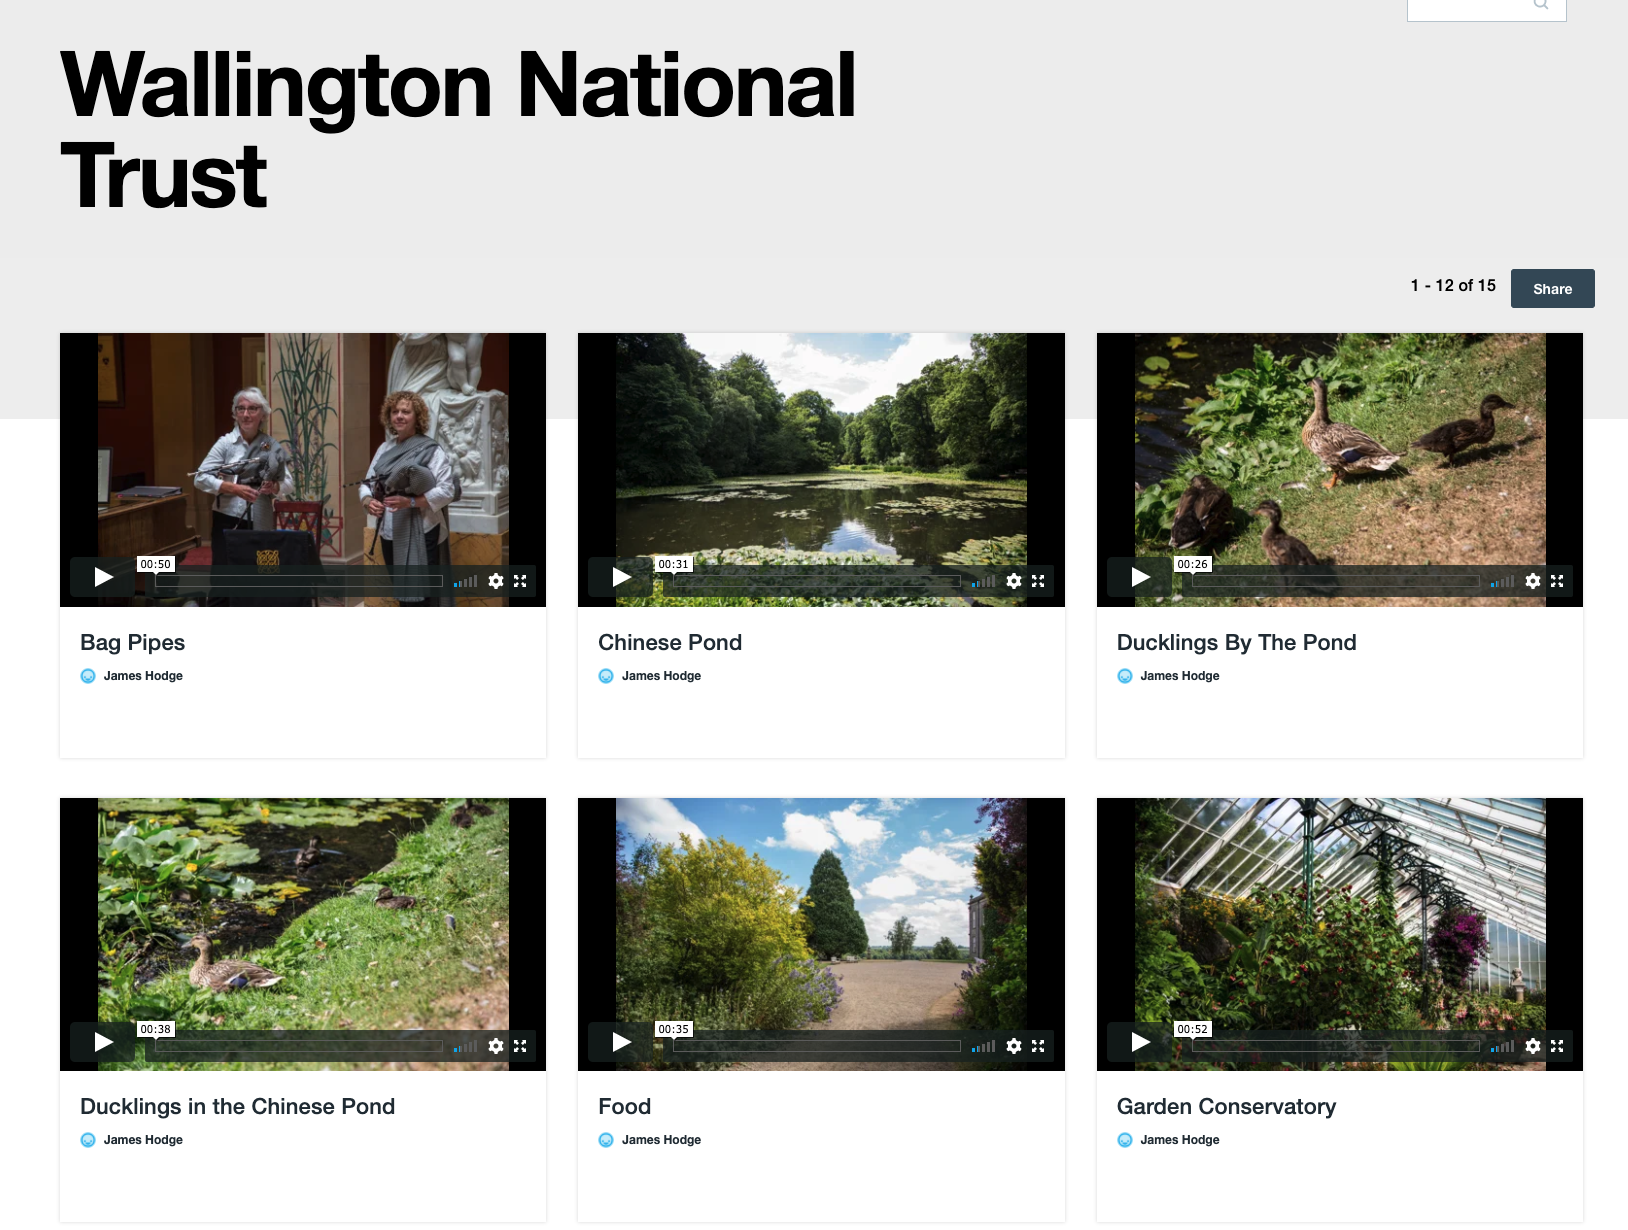
\includegraphics[width=.8\linewidth]{Images/ChapterFour/VimeoWebsite.png}
  \caption{Online archive on Vimeo}
  \label{fig:onlineArchive}
\end{subfigure}%
\begin{subfigure}{.5\textwidth}
  \centering
  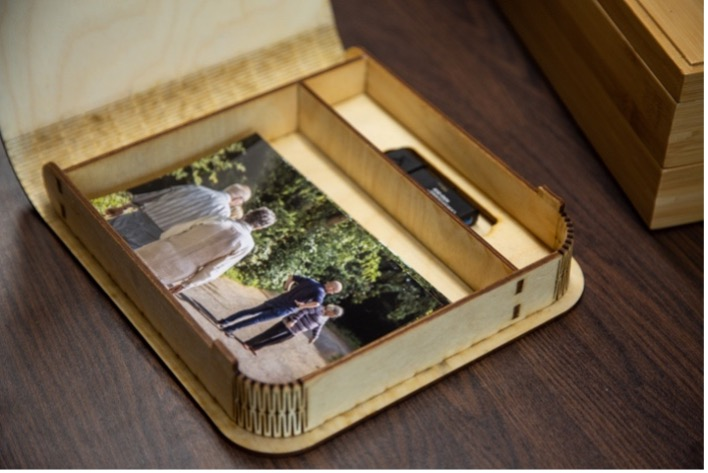
\includegraphics[width=.8\linewidth]{Images/ChapterFour/InsidePhotoAlbum.jpg}
  \caption{Album box with USB Stick}
  \label{fig:AlbumBox}
\end{subfigure}
\caption{Optional ways to access bespoke moments}
\label{fig:OptionalMoments}
\end{figure}

\section{Handing over the moment boxes}
\label{Relationships:HandingMomentBox}
In early April, I contacted Sarah, John, Lauren, and Michael to suggest a meeting for coffee and hand over the moment boxes. I tried to contact Kate and Philip through their daughters' email, but no luck in reaching out to them – later on, I found out they were going through some family problems. In mid-April, I arrived at Michael's house where I'd meet the four again. Michael and John were both at the door and welcomed me with open arms. I asked where Lauren and Sarah were, and they told me, "they're just chatting in the living room… We won't disturb them". With many carers reporting high levels of burnout and burden, John and Micheal's relationship was more than just a friendship, but also a distraction from their caregiving role. As we sat down and had a catch-up, I asked John how he was doing, and although I expected it, I was still sad to hear that the situation was no longer "we're lucky" or "life changing" as he had said just nine months ago. Instead, John echoed similarities to Michael's struggles that he was facing. John shared a story about how respecting Sarah's reality and going along with it as opposed to orienting her towards the 'right' reality:
\textit{
"It was about 2am couple days ago and I started to hear some banging downstairs… I walked downstairs and saw Sarah trying to open the front door. She told me she wanted to go home and I tried to get her to come back to bed but she wouldn't have any of it. Instead, she kept insisting this wasn't her home. I told her I'd take her home and we got in the car and I drove around for a bit and then we came back home and all was fine."
}
John acted in a way similar to the idea of eclipsing realities that has been discussed in this chapter but what I had not understood before, was some of the structural challenges of acting upon the 'dreamlike' state that someone living with dementia may be experiencing \citep{bryden_before_2015}. Although John often follows the 'Butterfly method' that focuses more on being in the moment as opposed to the ability to recall and recount memories \citep{hodge_exploring_2019}, he shared \textit{"it's tiring James... I'm constantly tired and was completely out of it the next day"}. Going along with what is classed as best practices do not necessarily make it any easier on the caregiver or the person living with dementia. Through the studies, I've seen participants change in personality and expression. After only nine months, I saw John's go from coping to expressing problems of finding self-care for himself. John's practice of care and Michael's may have differences when it came to orienting the person living with dementia or co-existing between realities, but as I write this, saying "Orienting the person with dementia towards the "right" reality has very little effect…It is also considered to be poor practice" \citep{hodge_exploring_2019} is easier said than done. Spending time in the area of dementia over the past few years, as I've had the luxury of being able to leave and reflect on the lived experiences of the participants, I've had a more in-depth understanding of how it may be challenging to see someone go through a diagnosis of dementia. 

Later on, I asked if Lauren and Sarah could come and see what I had made for the four of them. We all sat down together, and I got the boxes out and heard many expressions of excitement from the four. I placed the boxes between couples – one for Michael and Lauren and another for Sarah and John. They took the tops of the moment boxes, which revealed the personalised dioramas. Both of them expressed that they "love it" and started to feel and play with the grass and ducks in the ponds. After showing the album box with the photos from the days out, Michael asked, \textit{"What about the VR? I'm dying to try it"}. I took the VR headsets out, and we went over how to set them up and what the headset can do. John and Michael grabbed the headsets and placed them on together. As I directed them through the range of settings, they both started to talk and interact with one another as they explored the 360 experiences:

\begin{quote}
    
\textbf{John}: "here..Michael, are you seeing this? I see the house and you chatting to our James *laughter*

\textbf{Michael}: "Hang on a sec… I'm at the Ponds. Come to the ponds. How does he do that James?"

\textbf{James}: "Flick the top button of the controller in your hand and you'll start moving between the different 360 videos.

\textbf{John}: "Ah this is canny James"

\textbf{Michael}: "Look at the little chickens"
\end{quote}

At the time, Sarah and Lauren didn't seem too interested in the headsets. They were laughing at John and Michael's interactions alongside me. Unsurprisingly, this was expected from the prior study where participants mentioned a fear of looking foolish or looking silly when wearing the VR headsets \citep{hodge_exploring_2018} the 360 videos, I placed them on Vimeo – a video streaming service similar to YouTube. Michael and John had expressed earlier in the study that they had iPad's and would like to see the experiences using non-VR technology. I introduced the QR code activity and described it to the four. As Lauren and Sarah grabbed a random QR code albeit looking slightly unsure on what would happen, Michael and John scanned the code on their tablets and it opened a different 360 video. Lauren and Sarah could still drive the experience by rotating the camera with finger gestures on the screen. With the tutorial guides I had place in the box and my introduction of the technology to the families, I had hoped for the families to return to the future experiences. A couple of weeks later, I had a brief call with John and Michael about their interactions with the moment boxes. Sarah and Lauren both had spent very little time experiencing any of the VR experiences but would sometimes sit down and play with the dioramas, the photos and playing with the QR code 'lines. Sarah found the burnt lines into the plywood to create the QR code interesting to feel and hold. For Michael and John, they felt guilty that what I had made wasn't being used as much. As we discussed that this would be the end of the study, both thanked me for all the work and said, "\textit{if you are ever doing this again… we'd be more than happy to go on another day out"}.

While the families were thankful, their comments suggested that VR wasn't a technology they felt comfortable with or were wanting to explore anymore. A key issue discussed in the HCI community is a push for innovative projects. Meurer et al. discuss the problems of innovation and its impacts on sustainability \citep{meurer_designing_2018}. Involving VR from a research perspective and Sandra's for the dementia café put pressure on time and resources to explore a technology that may not be appropriate for the community. VR technology has come a long way but still isn't quite there. Personally, I've seen rapid development of VR headsets becoming more user-friendly. As Facebook has started to develop headsets that the families used, they have become far more accessible and useable since 2017. Vine et al. describe ethical difficulties in using Google Glass, supported by Google, which still had bugs typically found in prototypes (\citep{vines_our_2017}. Although the Oculus Go Headset, and Google Glass – both supported by large corporations, their user interfaces and uses are continued to be designed for the majority instead of the marginalised. Michael expressed a struggle to navigate the system after I wasn't there to direct him through the step-by-step guide. Even though I had written them down, a paper tutorial is far more difficult to use while you're navigating a VR interface. Despite failures of longevity in the families wanting to use VR, they remained thankful and would be more than 'happy' to participate in any similar study. The families expressed to take part in similar studies resonated with the impact being less about the technology, but rather the involvement and opportunities for meaningful engagement. Wallace et al. expresses the impact through the relationships and involvement created between the study and the participant. Wallace discusses how involving her participants as the driving point, the study itself became important to them. Furthermore, documenting the process with photos for the family, the images held significant value to the participants \citep{wallace_design-led_2013}. 

\section{Summary}
\label{Relationships:Summary}
In this chapter, I have provided reflective insights into three years worth of research where I worked closely with people with dementia and their family members. The focus of the reflection aimed to shed light on the implications of conducting participatory design within this space. In turn, the chapter raises conflicting problems in balancing study expectations with research partners; ' ethical protectionism' employed by Ethical Review Boards preventing later stages of dementia participating; and the value of the researcher-participant relationship. Although, as researchers in the field, we may understand that every person has personhood, this doesn't always seem apparent in the real world. As researchers, our next steps are to consider what it means to be an inclusive society, what it means to do inclusive research and to question the infrastructures that surround and often hold up our work. For instance, as researchers, how can we ensure ethical review boards are reflexive and dynamic when they are evaluating research that seeks to design in sensitive settings? Likewise, while HCI and dementia has explored the nuances and importance of relational approaches in developing technology with people with dementia, understanding how these interactions may scale between people with dementia and designers and developers remains underexamined.

Finally, when we consider our impact, it is essential to note that technology offers opportunities for meaningful engagement as well as create challenges relating to robustness and longevity when the project ends. Typical strategies to overcome these challenges could be to ensure a longer lifespan and technology support if anything goes wrong. Alternatively, we can aim for technology to become a part of a community and create meaningful relationships with our participant groups and research ecologies. This pertains to participatory and community-based research, personalisation, recognition and meaning. In this way, it's clear that technology alone does not hold any value; it's the relationships and experiences it creates and mediates.

\begin{figure}[htp]
\centering
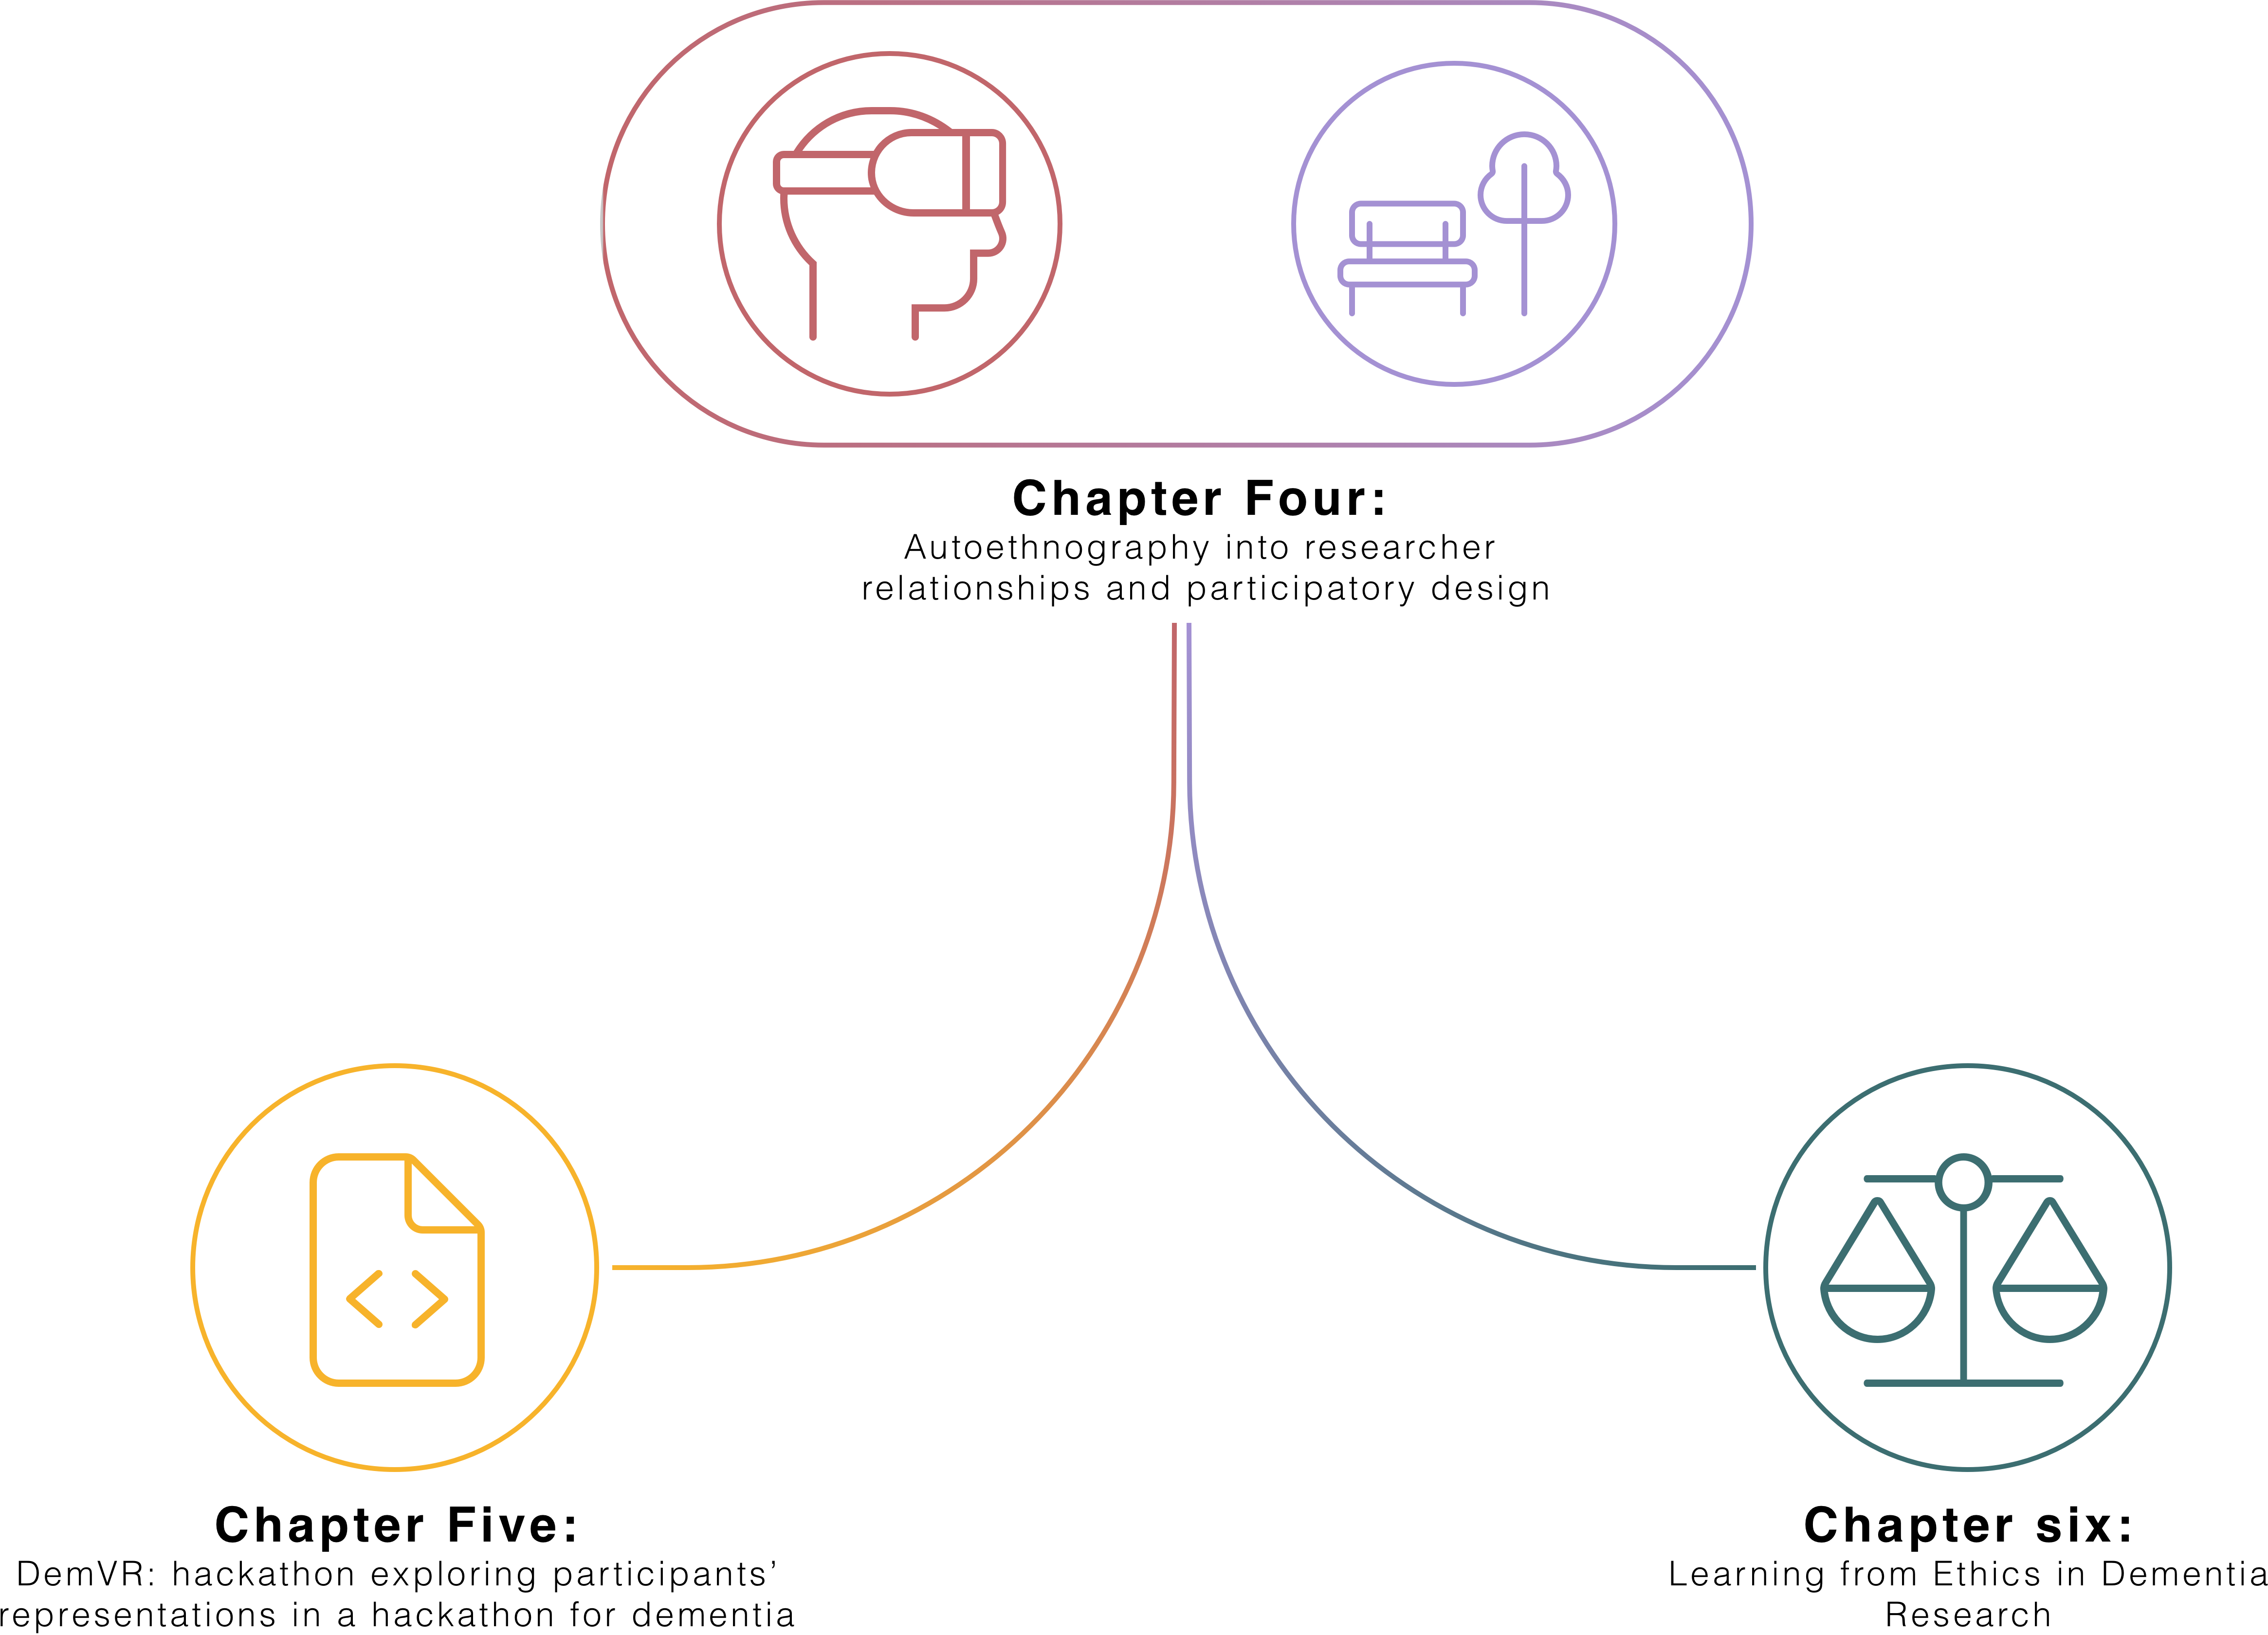
\includegraphics[width=0.6\linewidth]{Images/Thesis_Narrative/Narrative_ChapterFour.png}
\caption{Subsequent chapters}
\label{fig:ChapterFour_FutureStudies}
\end{figure}

The two distinct themes from this work that need additional consideration are the following:
\begin{enumerate}

    \item Explore the role of participation between people with dementia, developers and designers in public engagement 
    \item To examine the impact of research ethics on participatory approaches in dementia from a researcher's perspective
\end{enumerate}

In response to these developed themes, the following two data chapters highlighted in fig.\ref{fig:ChapterFour_FutureStudies} study the themes in more detail to broaden the conversation on dementia and HCI to other stakeholders that influence the relationship between technology and people with dementia. In the next chapter, we start with the first theme that provides deep insights into the shifting representations of dementia in a hackathon that seeks to provide a creative and inclusive space for the public to engage on dementia.
